\chapter{Convergence of SLI global parameters in JICF}
\label{app:SLI_convergence}

Spray characterization from the JICF simulations of Chapter has been presented in $\S$\ref{subsec:ch5_sec_spray_characterization}: the total accumulation times of the simulations are summarized in Table \ref{tab:jicf_SLI_t_prime_accumulation} and the amount of accumulated droplets in Table \ref{tab:jicf_SLI_Ndr_accumulated}. The establishment of the sprays was shown through the convergence of the global SMD and liquid flux $Q_l$ in Figure \ref{fig:ch5_spray_char_establishment}. In this section, the convergence on the remaining parameters not previously shown are displayed: velocities in three directions are shown in Figures \ref{fig:app_spray_velocities_establishment_mean} and \ref{fig:app_spray_velocities_establishment_rms}, and deformation parameters $\alpha$ and $\beta$ are seen in Figures \ref{fig:app_spray_deformation_establishment_mean} and \ref{fig:app_spray_deformation_establishment_rms}.


\clearpage

\subsection*{Liquid velocities}

\begin{figure}[ht]
	\centering
   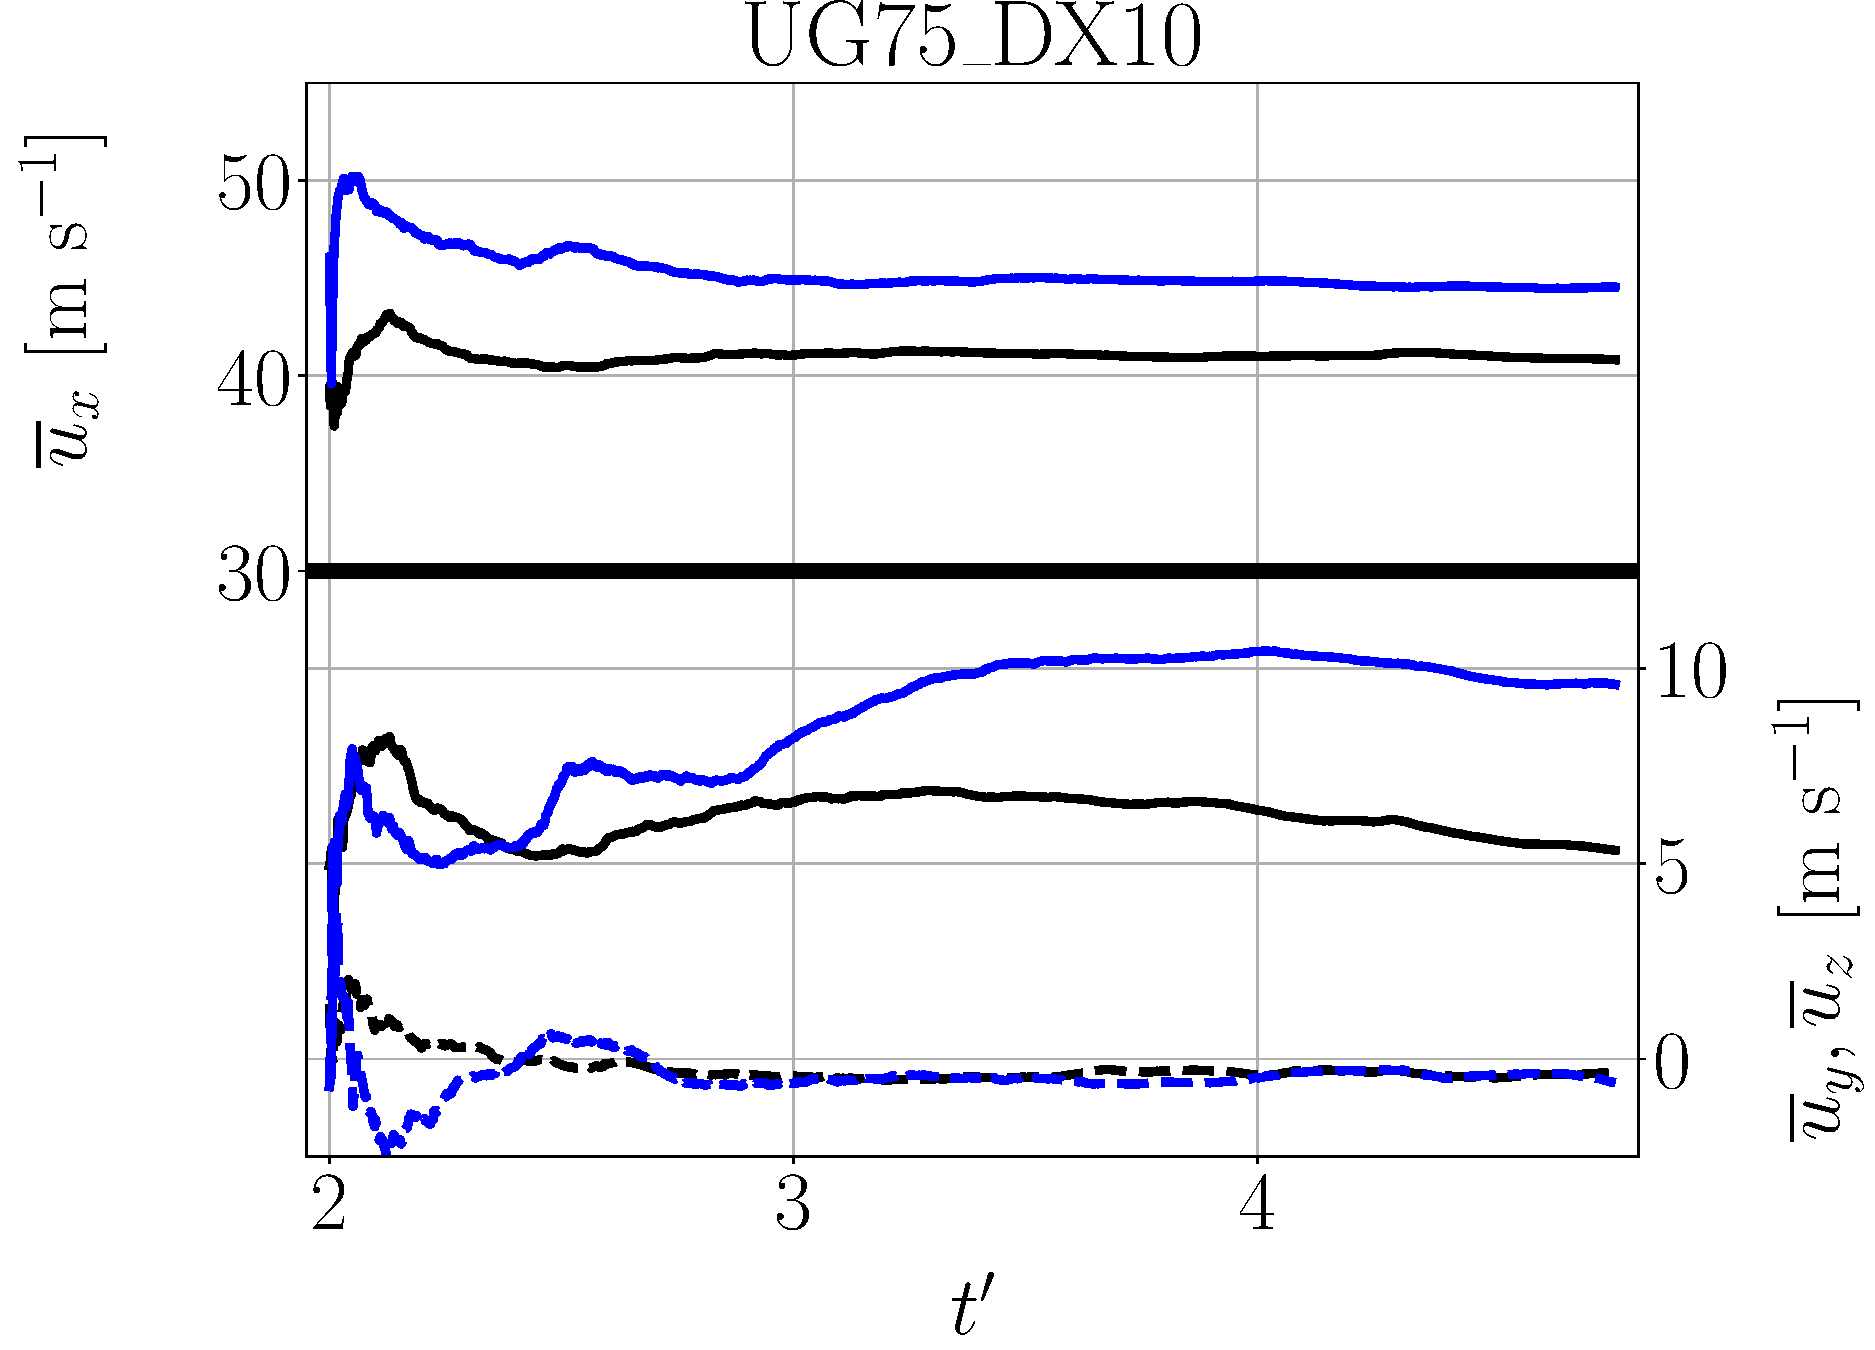
\includegraphics[width=0.3\textwidth]{./part2_developments/figures_ch5_resolved_JICF/SPRAY_characterization/velocities_establishment/establishment_UG75_DX10_mean}
   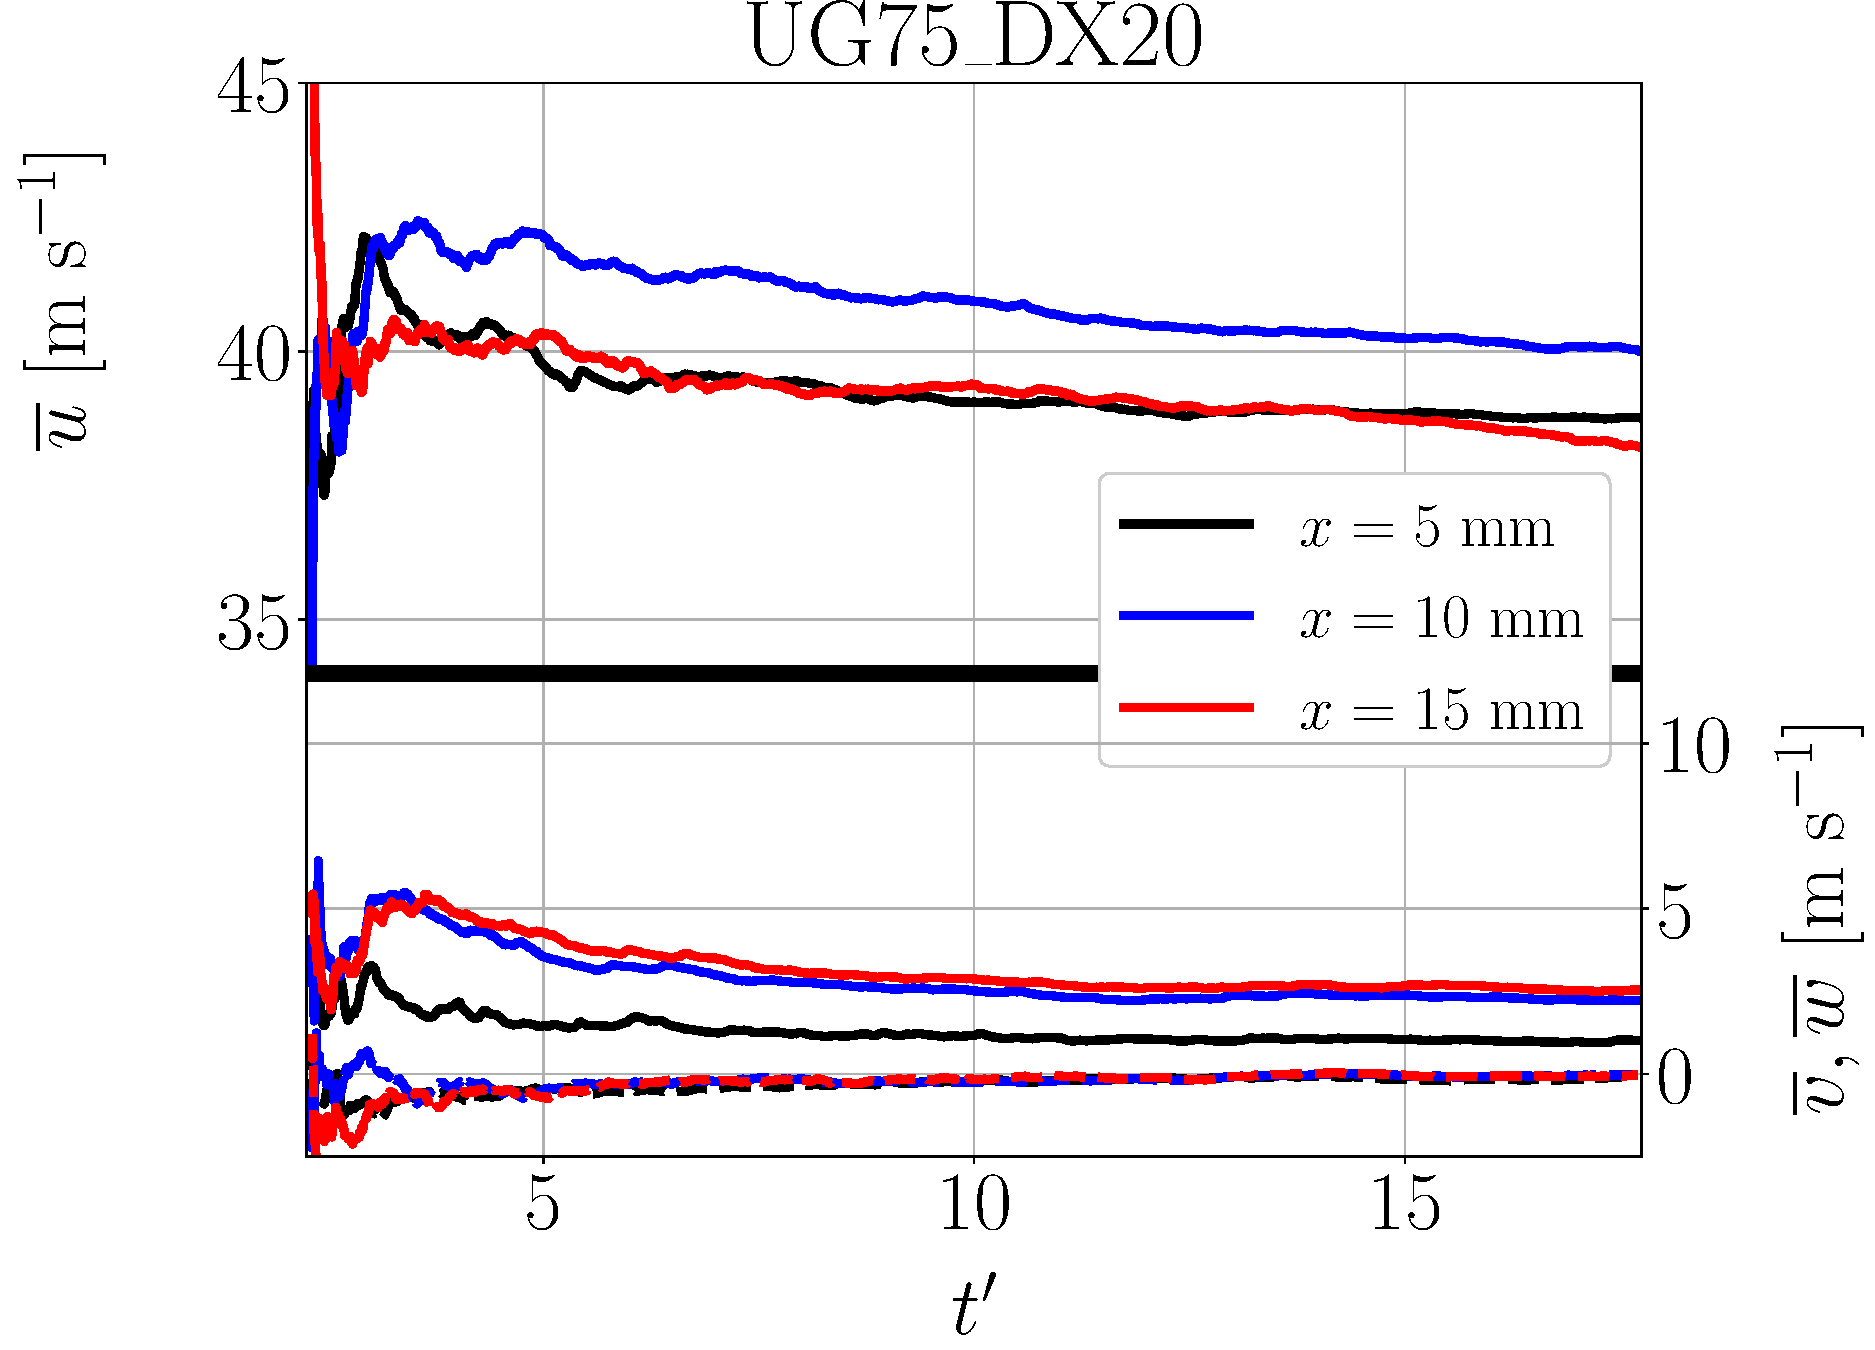
\includegraphics[width=0.3\textwidth]{./part2_developments/figures_ch5_resolved_JICF/SPRAY_characterization/velocities_establishment/establishment_UG75_DX20_mean}
   
	\vskip\baselineskip
	
   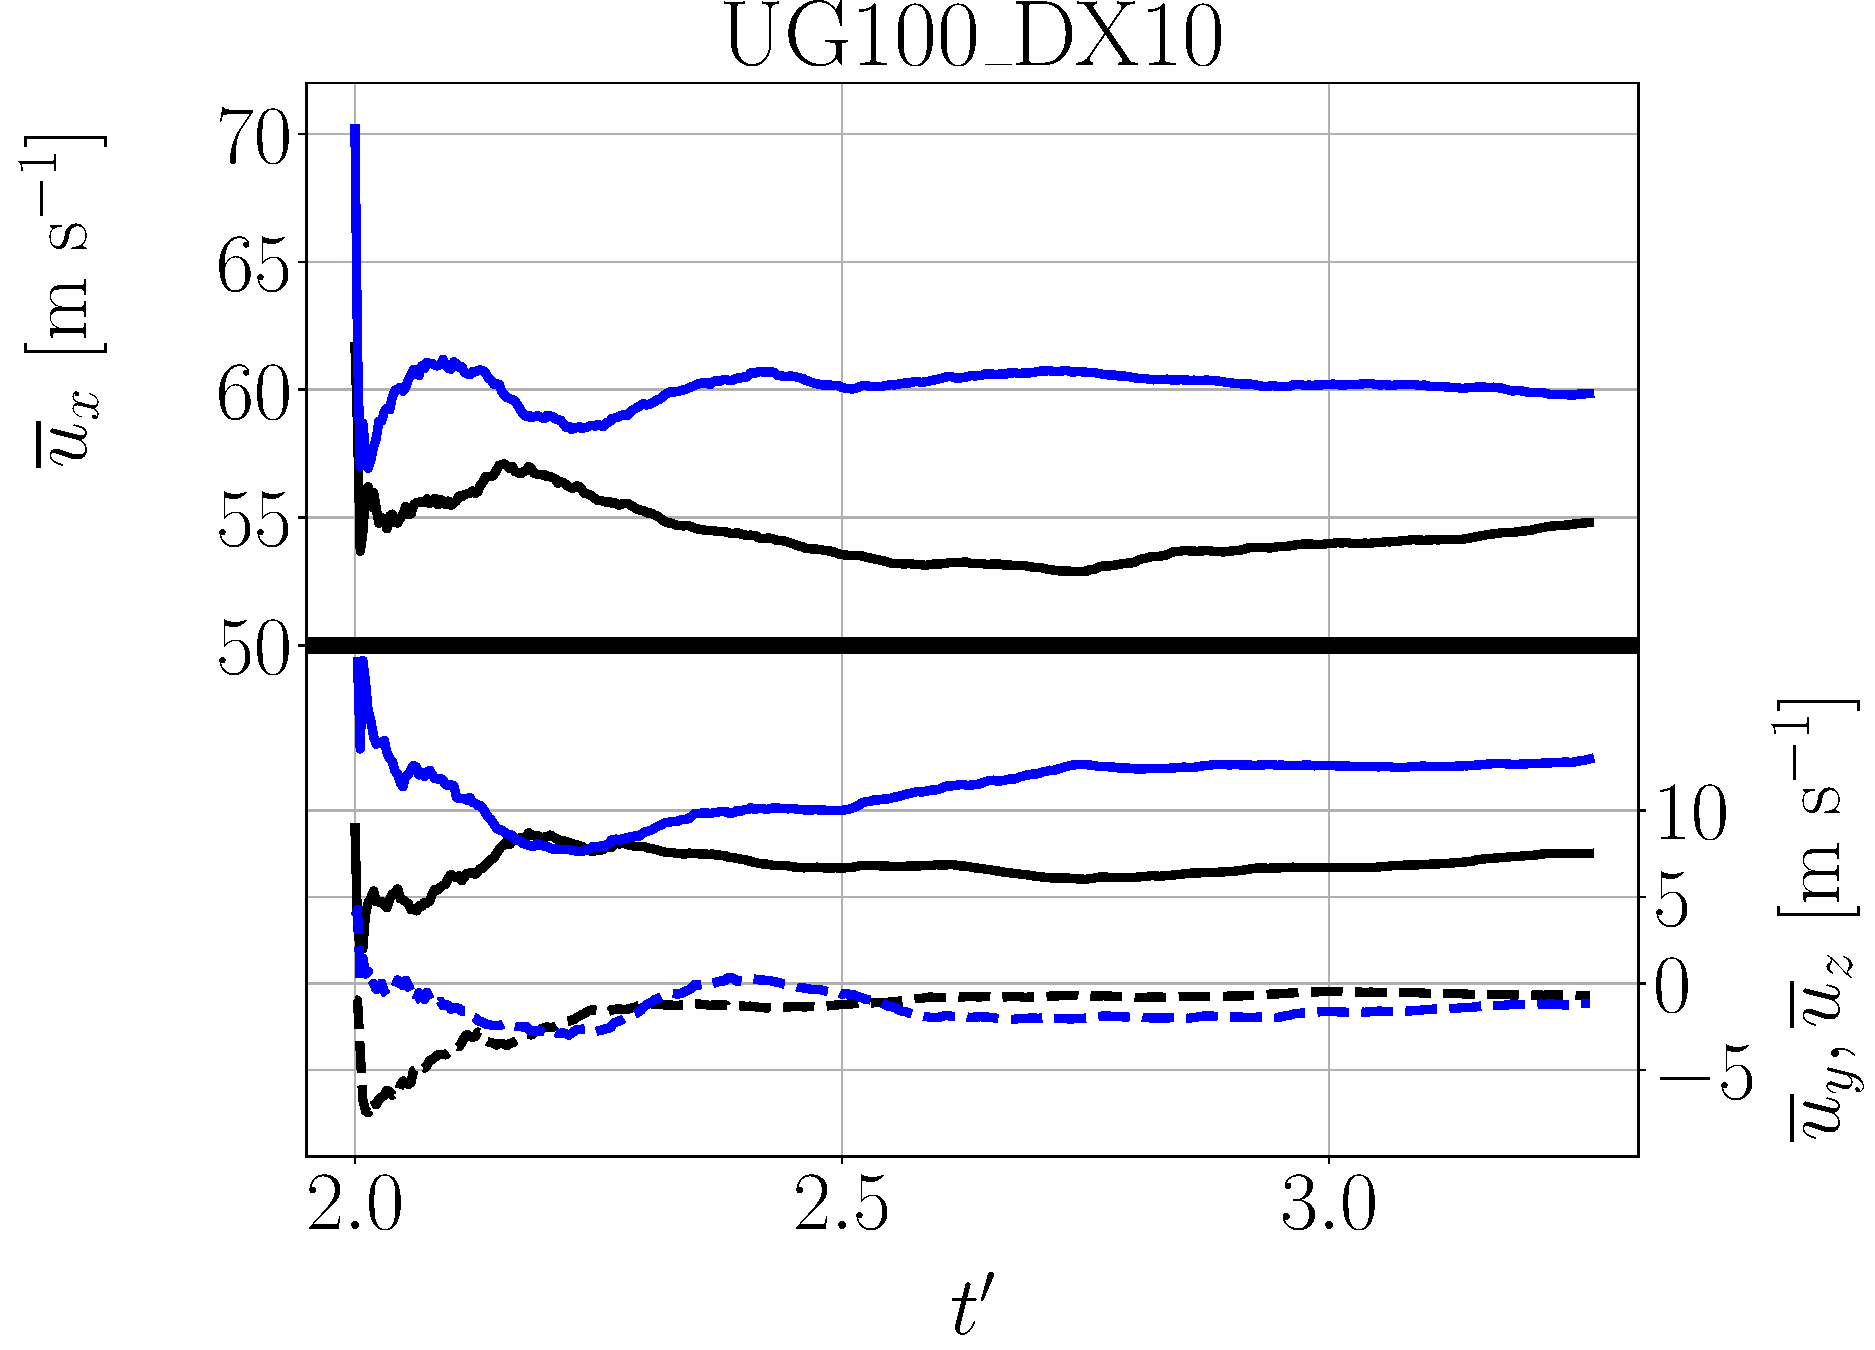
\includegraphics[width=0.3\textwidth]{./part2_developments/figures_ch5_resolved_JICF/SPRAY_characterization/velocities_establishment/establishment_UG100_DX10_mean}
   \hspace*{-0.1in}
   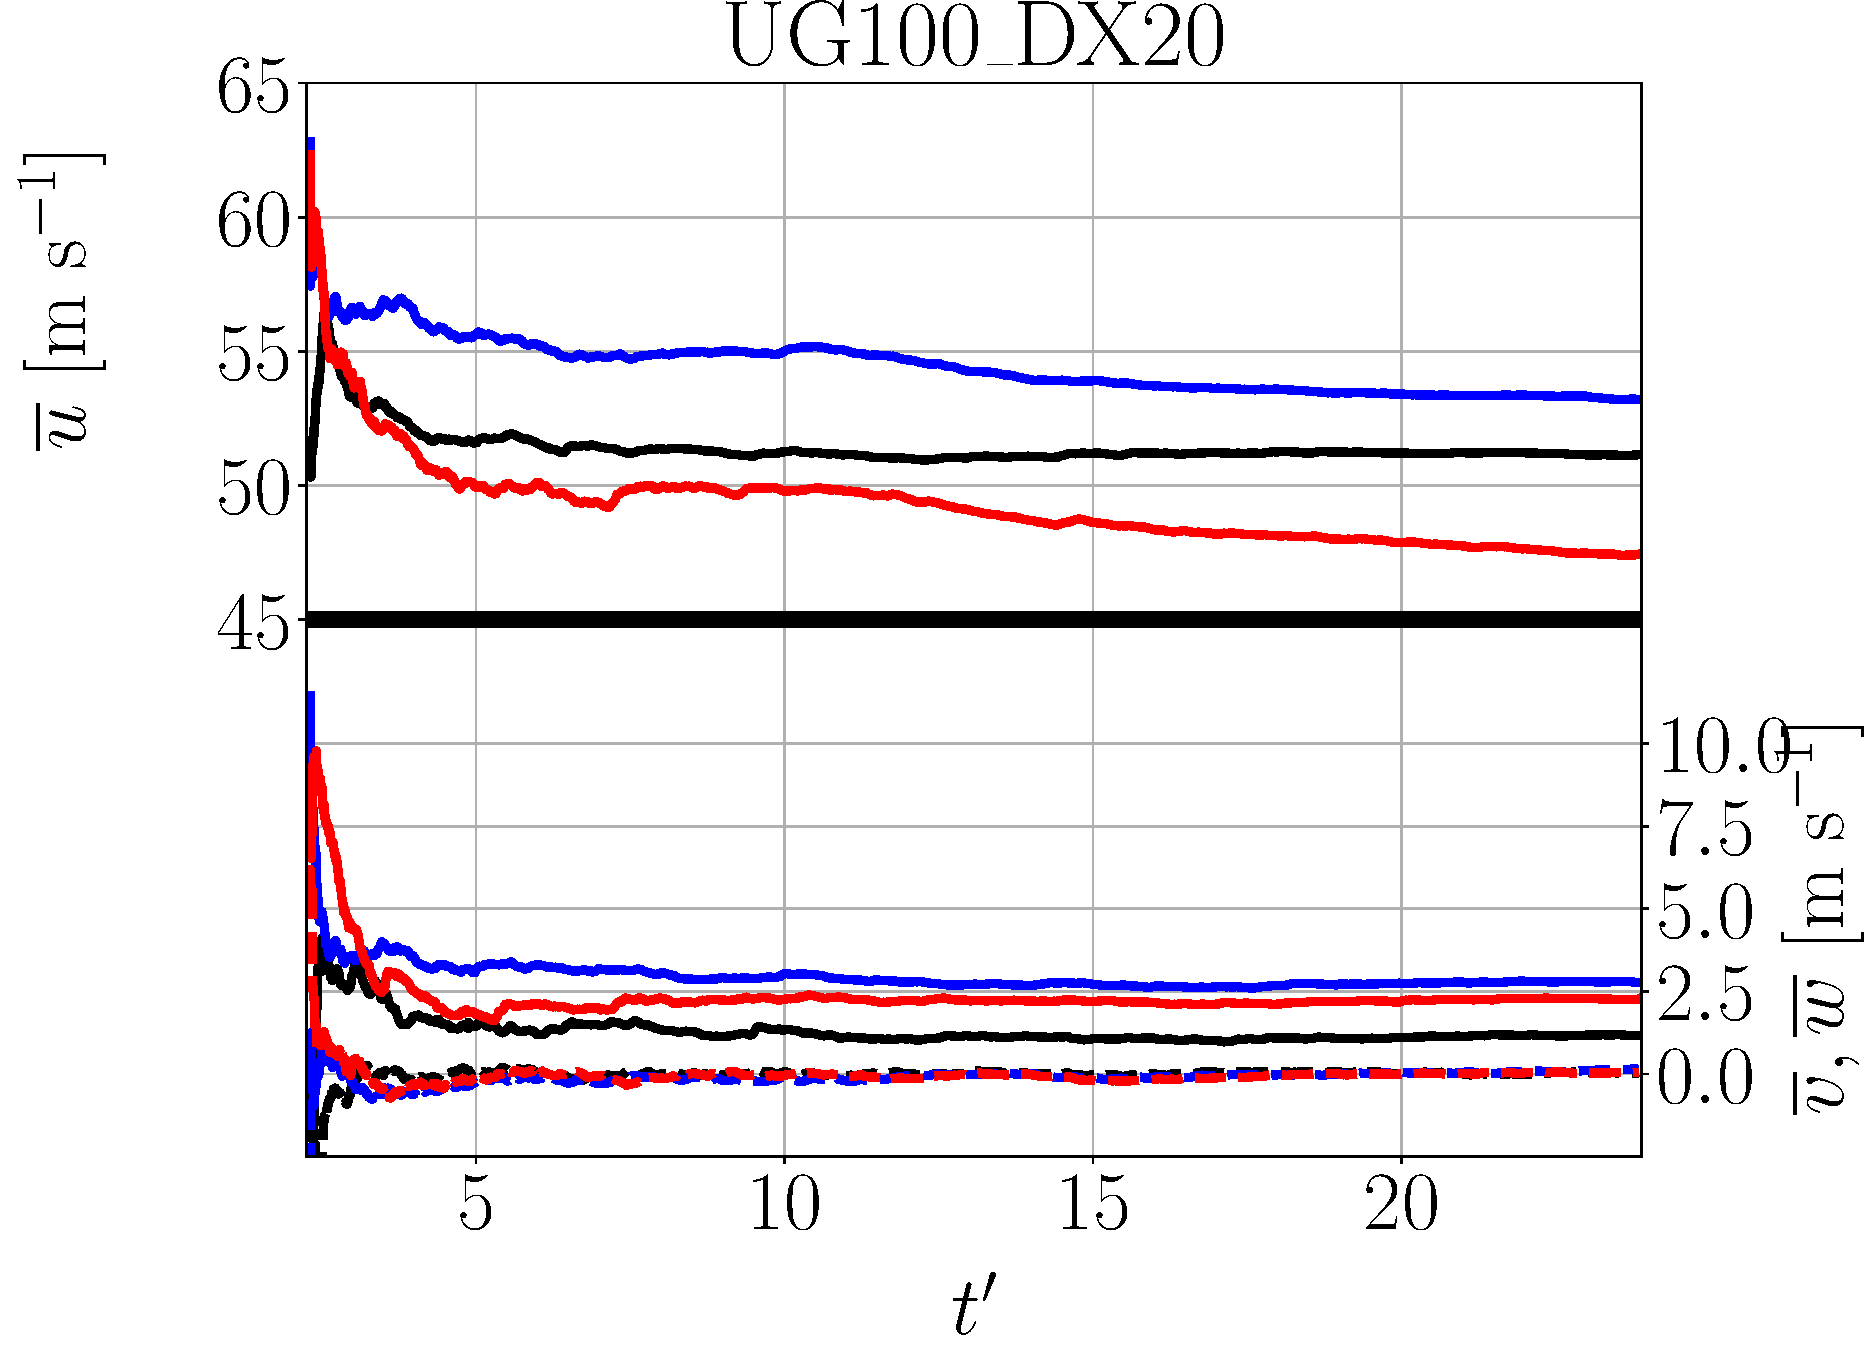
\includegraphics[width=0.3\textwidth]{./part2_developments/figures_ch5_resolved_JICF/SPRAY_characterization/velocities_establishment/establishment_UG100_DX20_mean}
   \hspace*{-0.1in}
   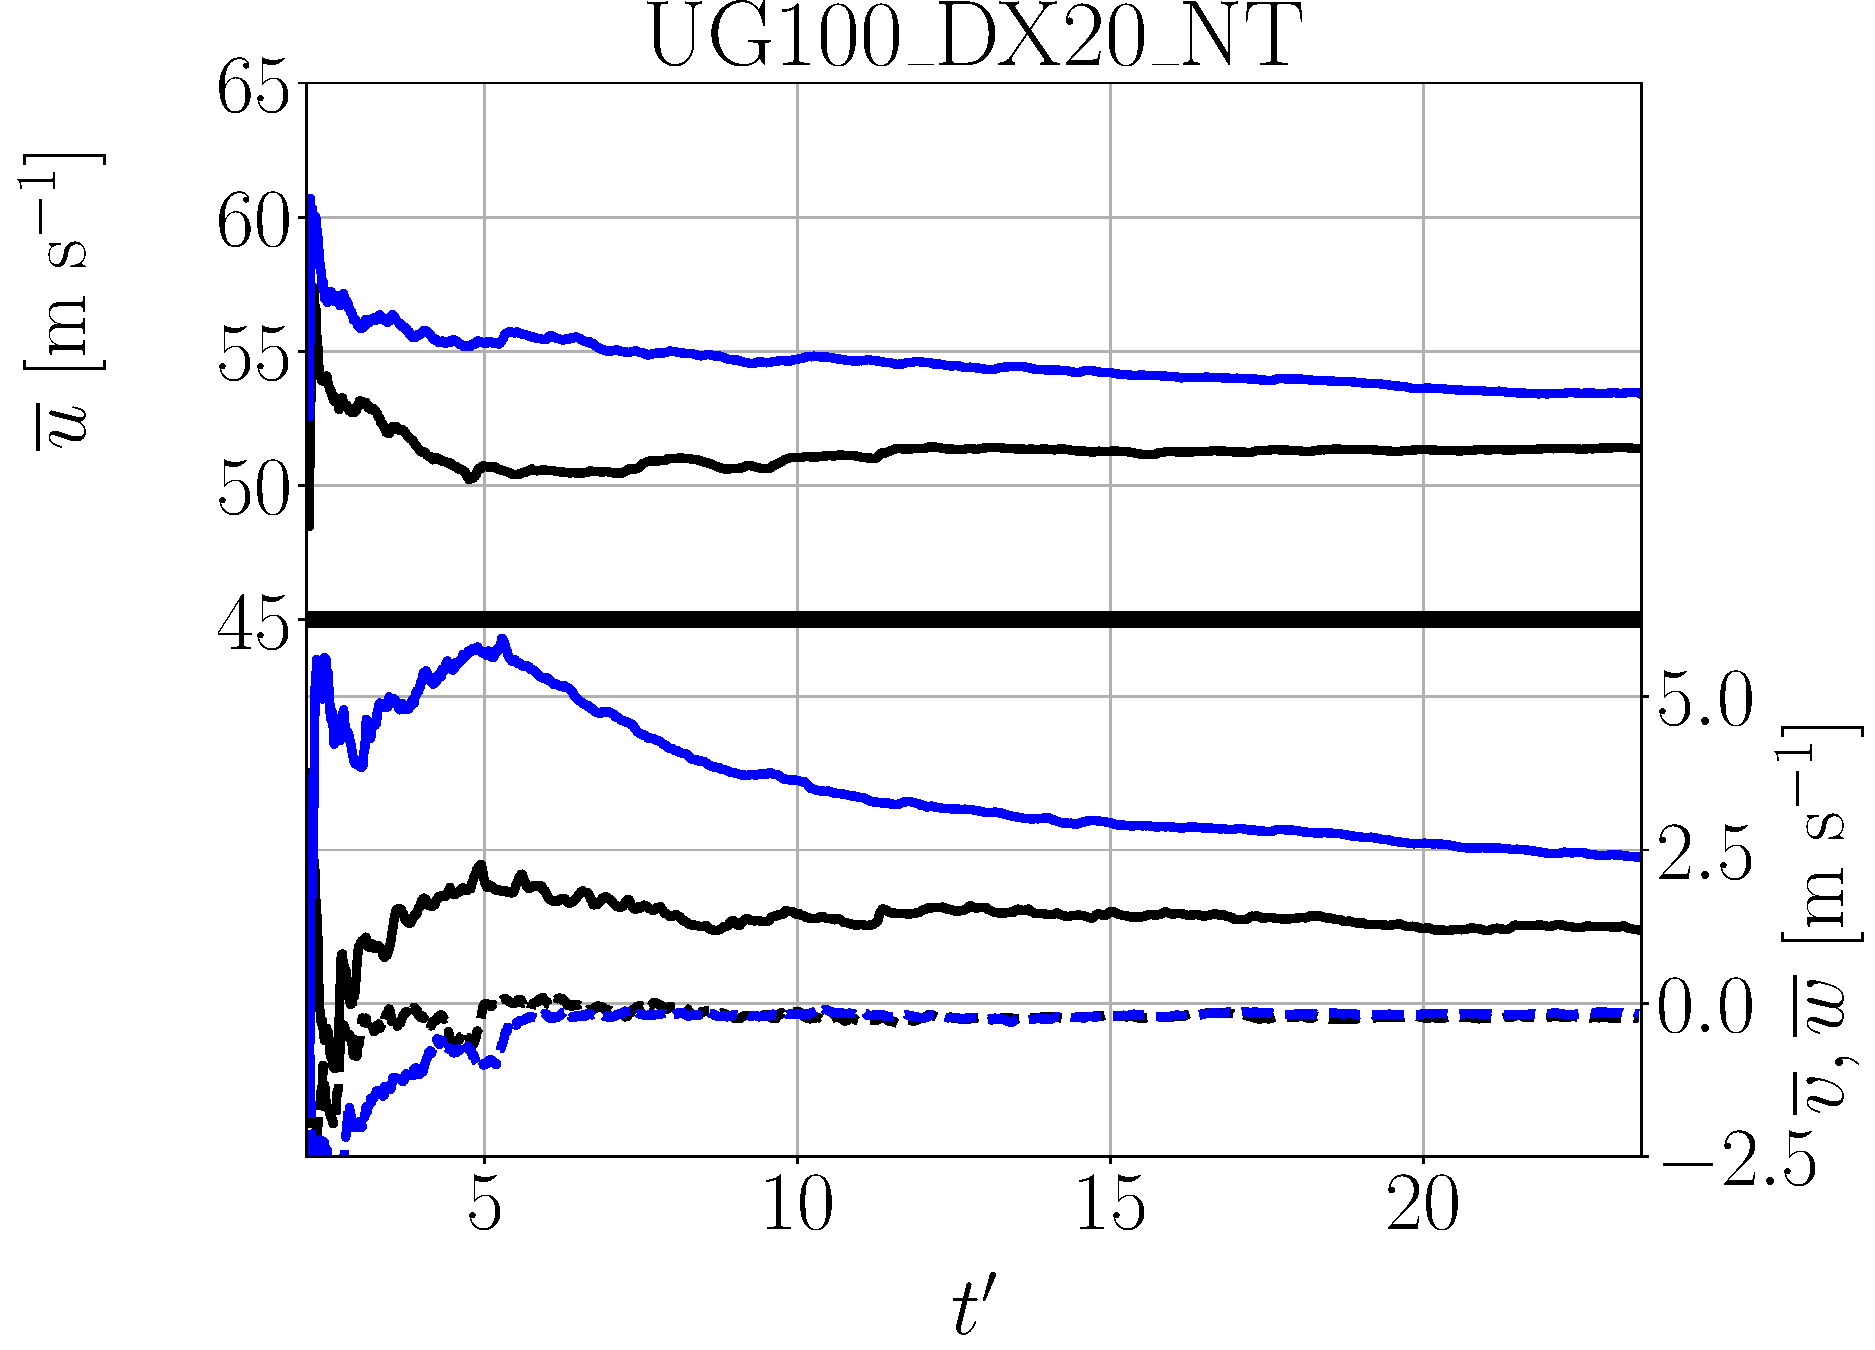
\includegraphics[width=0.3\textwidth]{./part2_developments/figures_ch5_resolved_JICF/SPRAY_characterization/velocities_establishment/establishment_UG100_DX20_NT_mean}
   \caption{Establishment of mean liquid velocities for each case.}
\label{fig:app_spray_velocities_establishment_mean}
\end{figure}

\vspace*{0.2in}

\begin{figure}[ht]
	\centering
   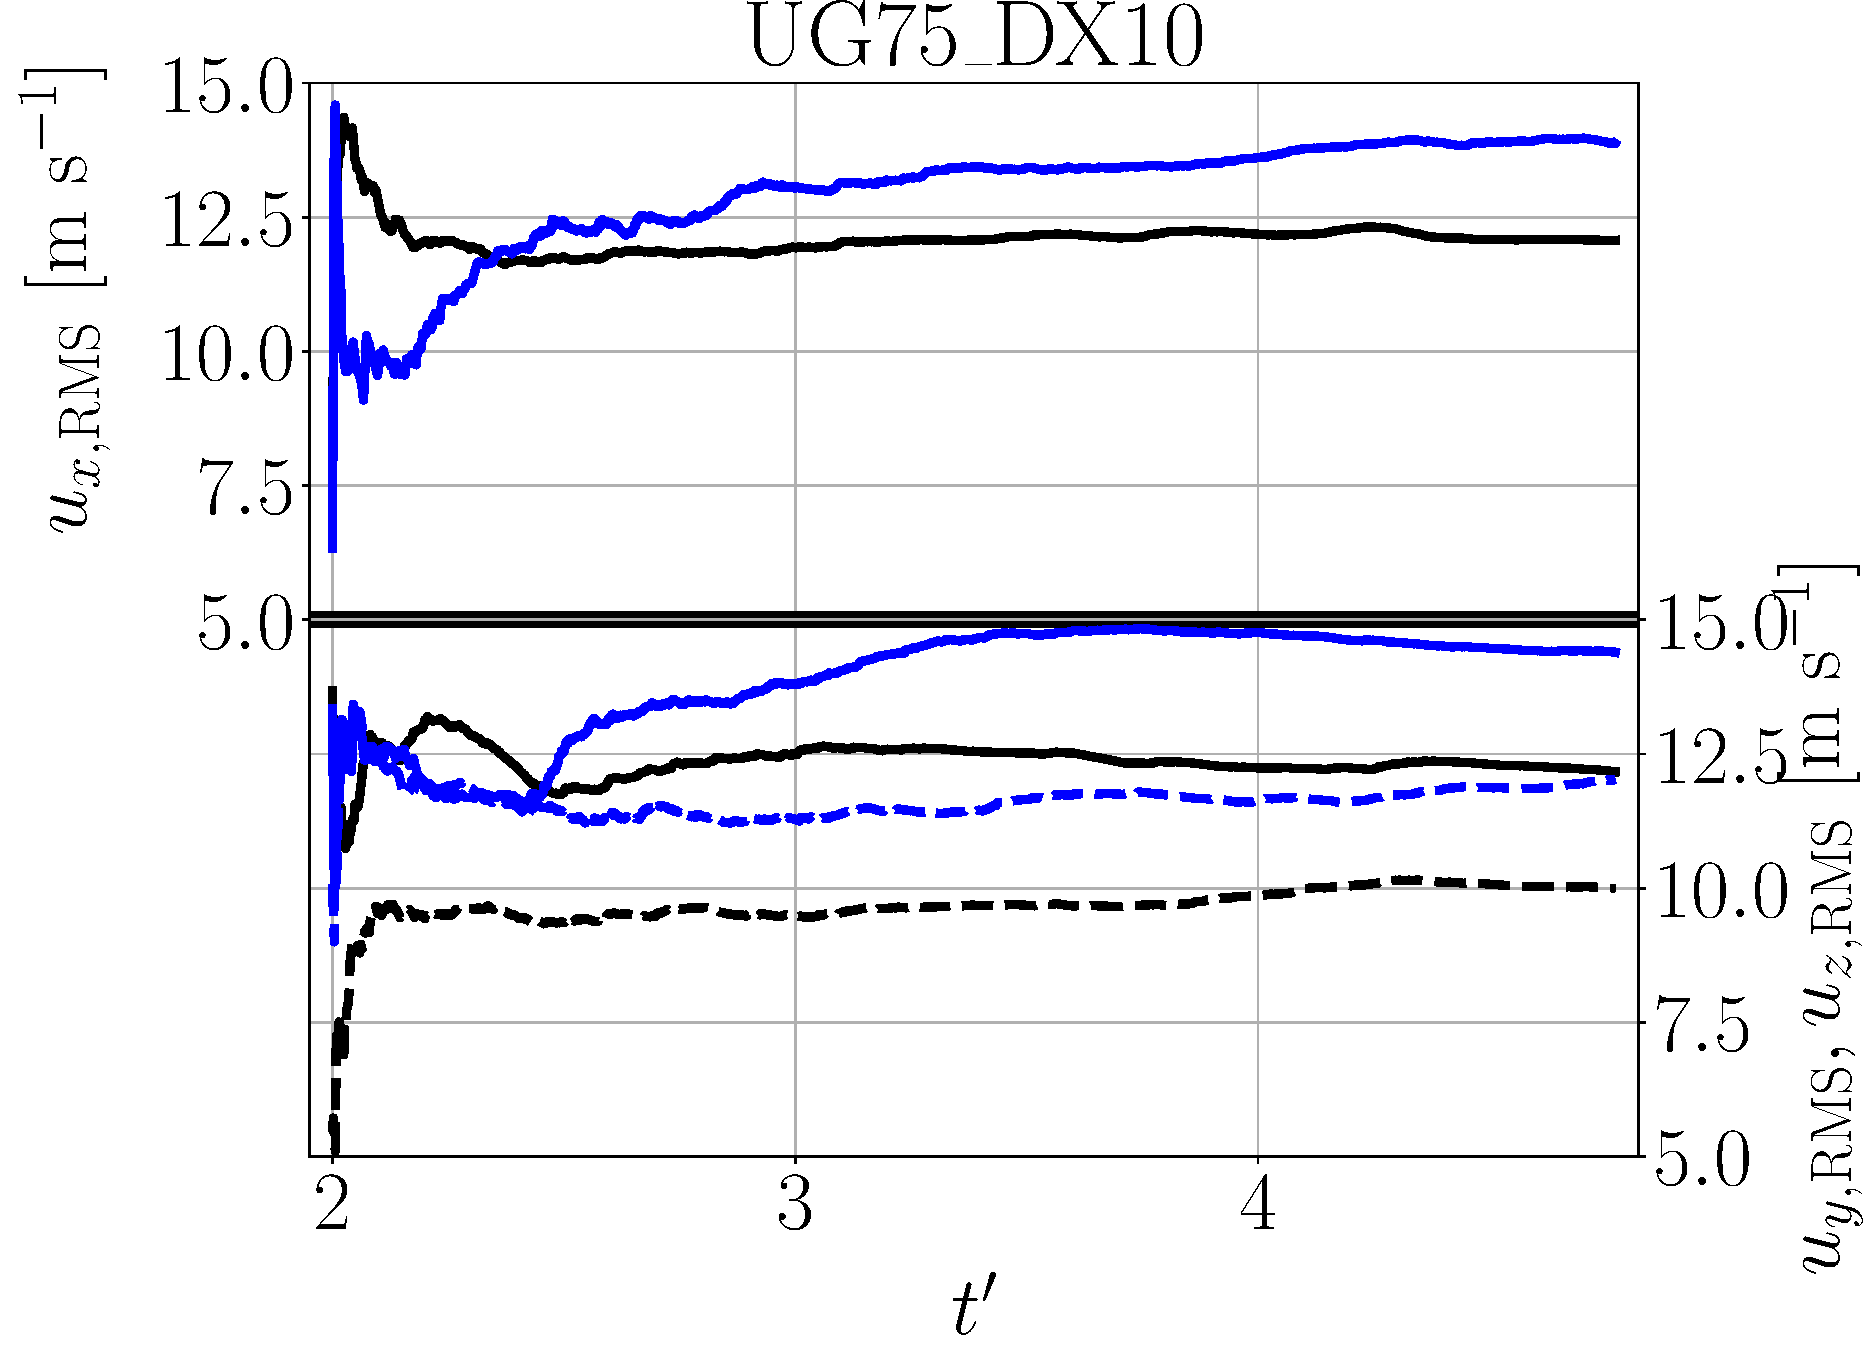
\includegraphics[width=0.3\textwidth]{./part2_developments/figures_ch5_resolved_JICF/SPRAY_characterization/velocities_establishment/establishment_UG75_DX10_rms}
   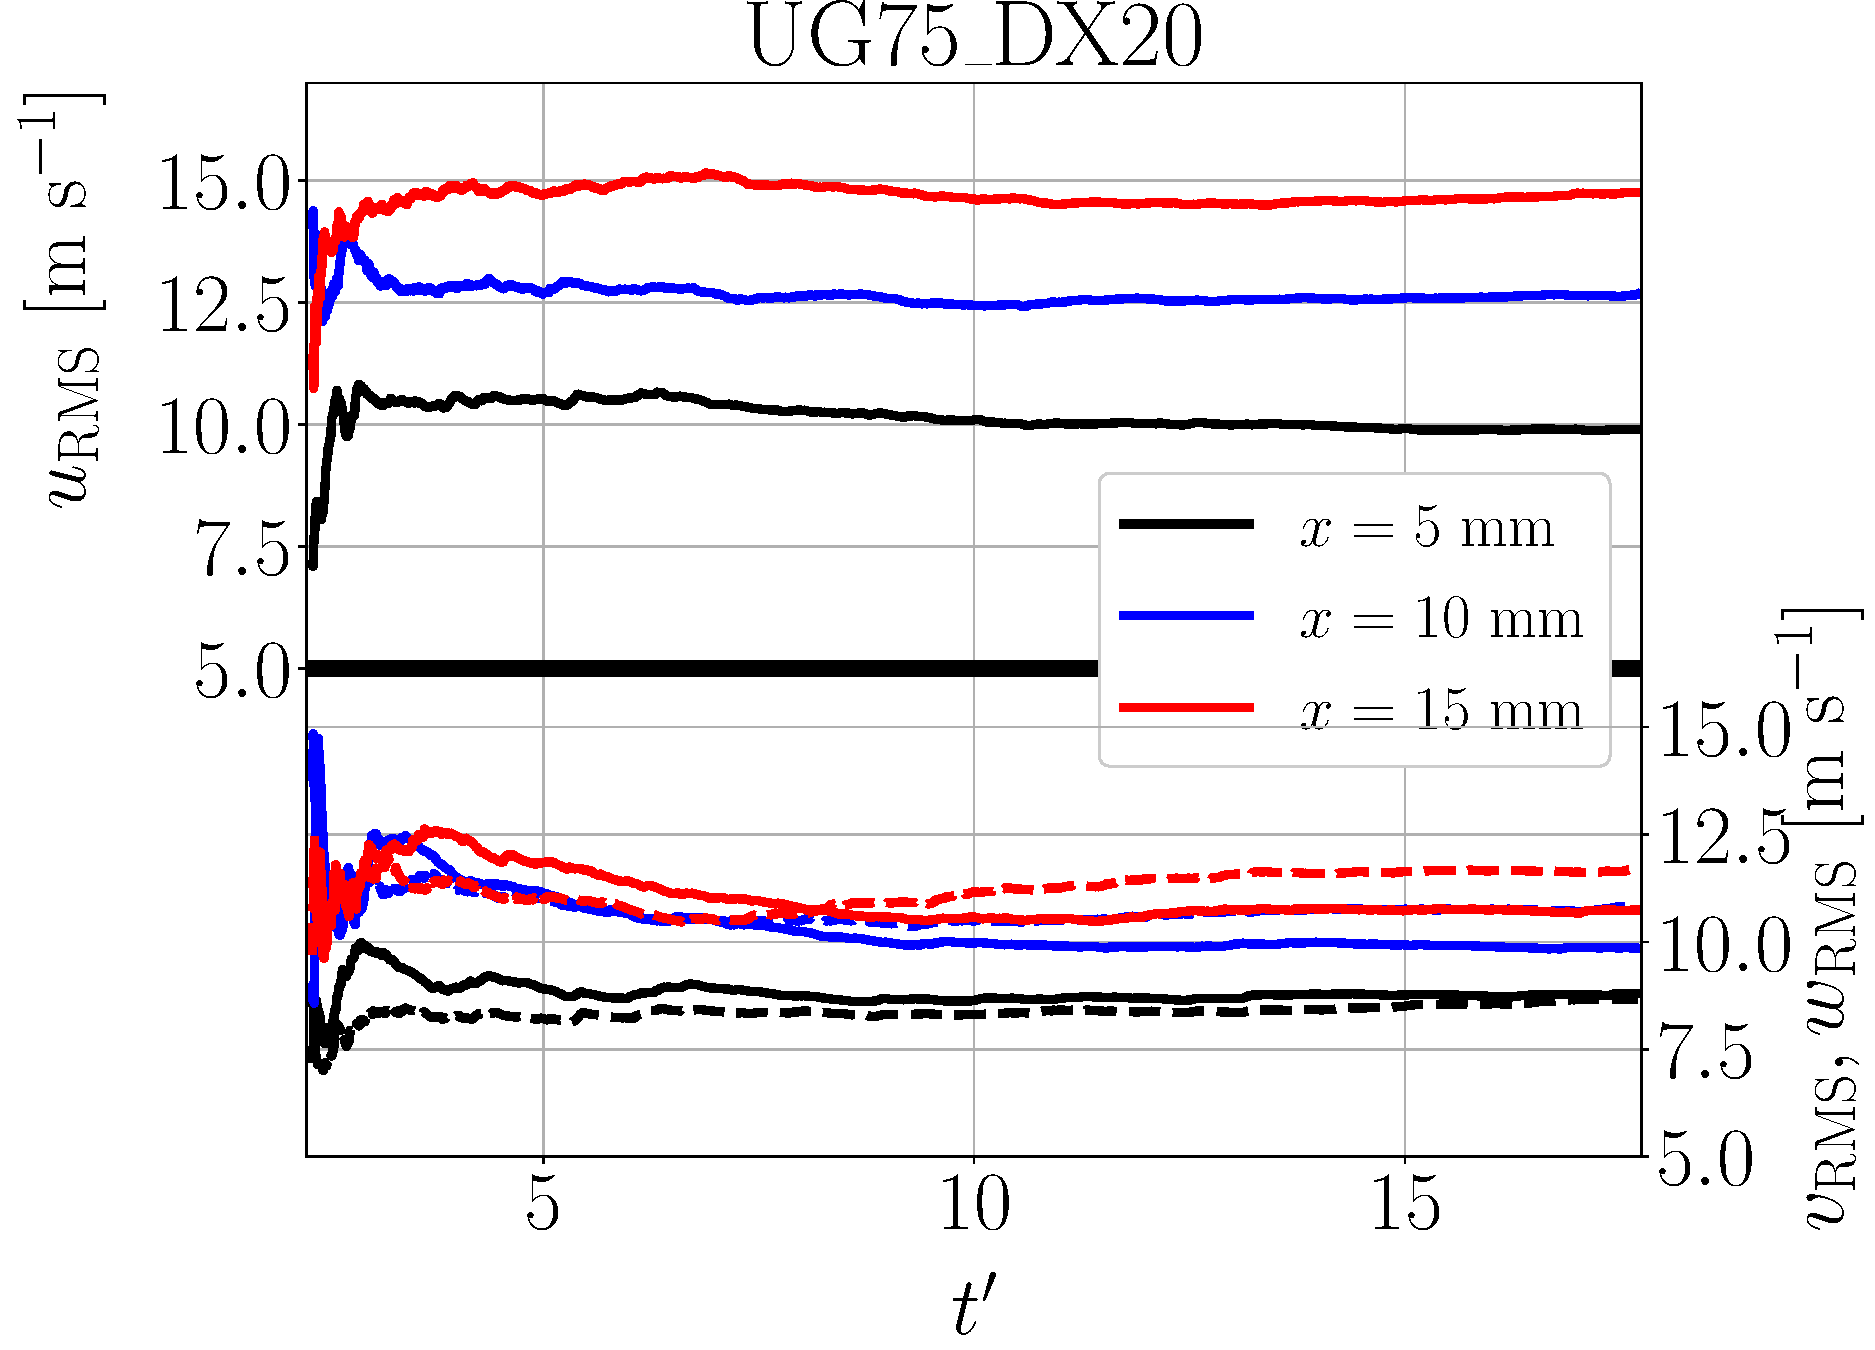
\includegraphics[width=0.3\textwidth]{./part2_developments/figures_ch5_resolved_JICF/SPRAY_characterization/velocities_establishment/establishment_UG75_DX20_rms}
   
	\vskip\baselineskip
	
   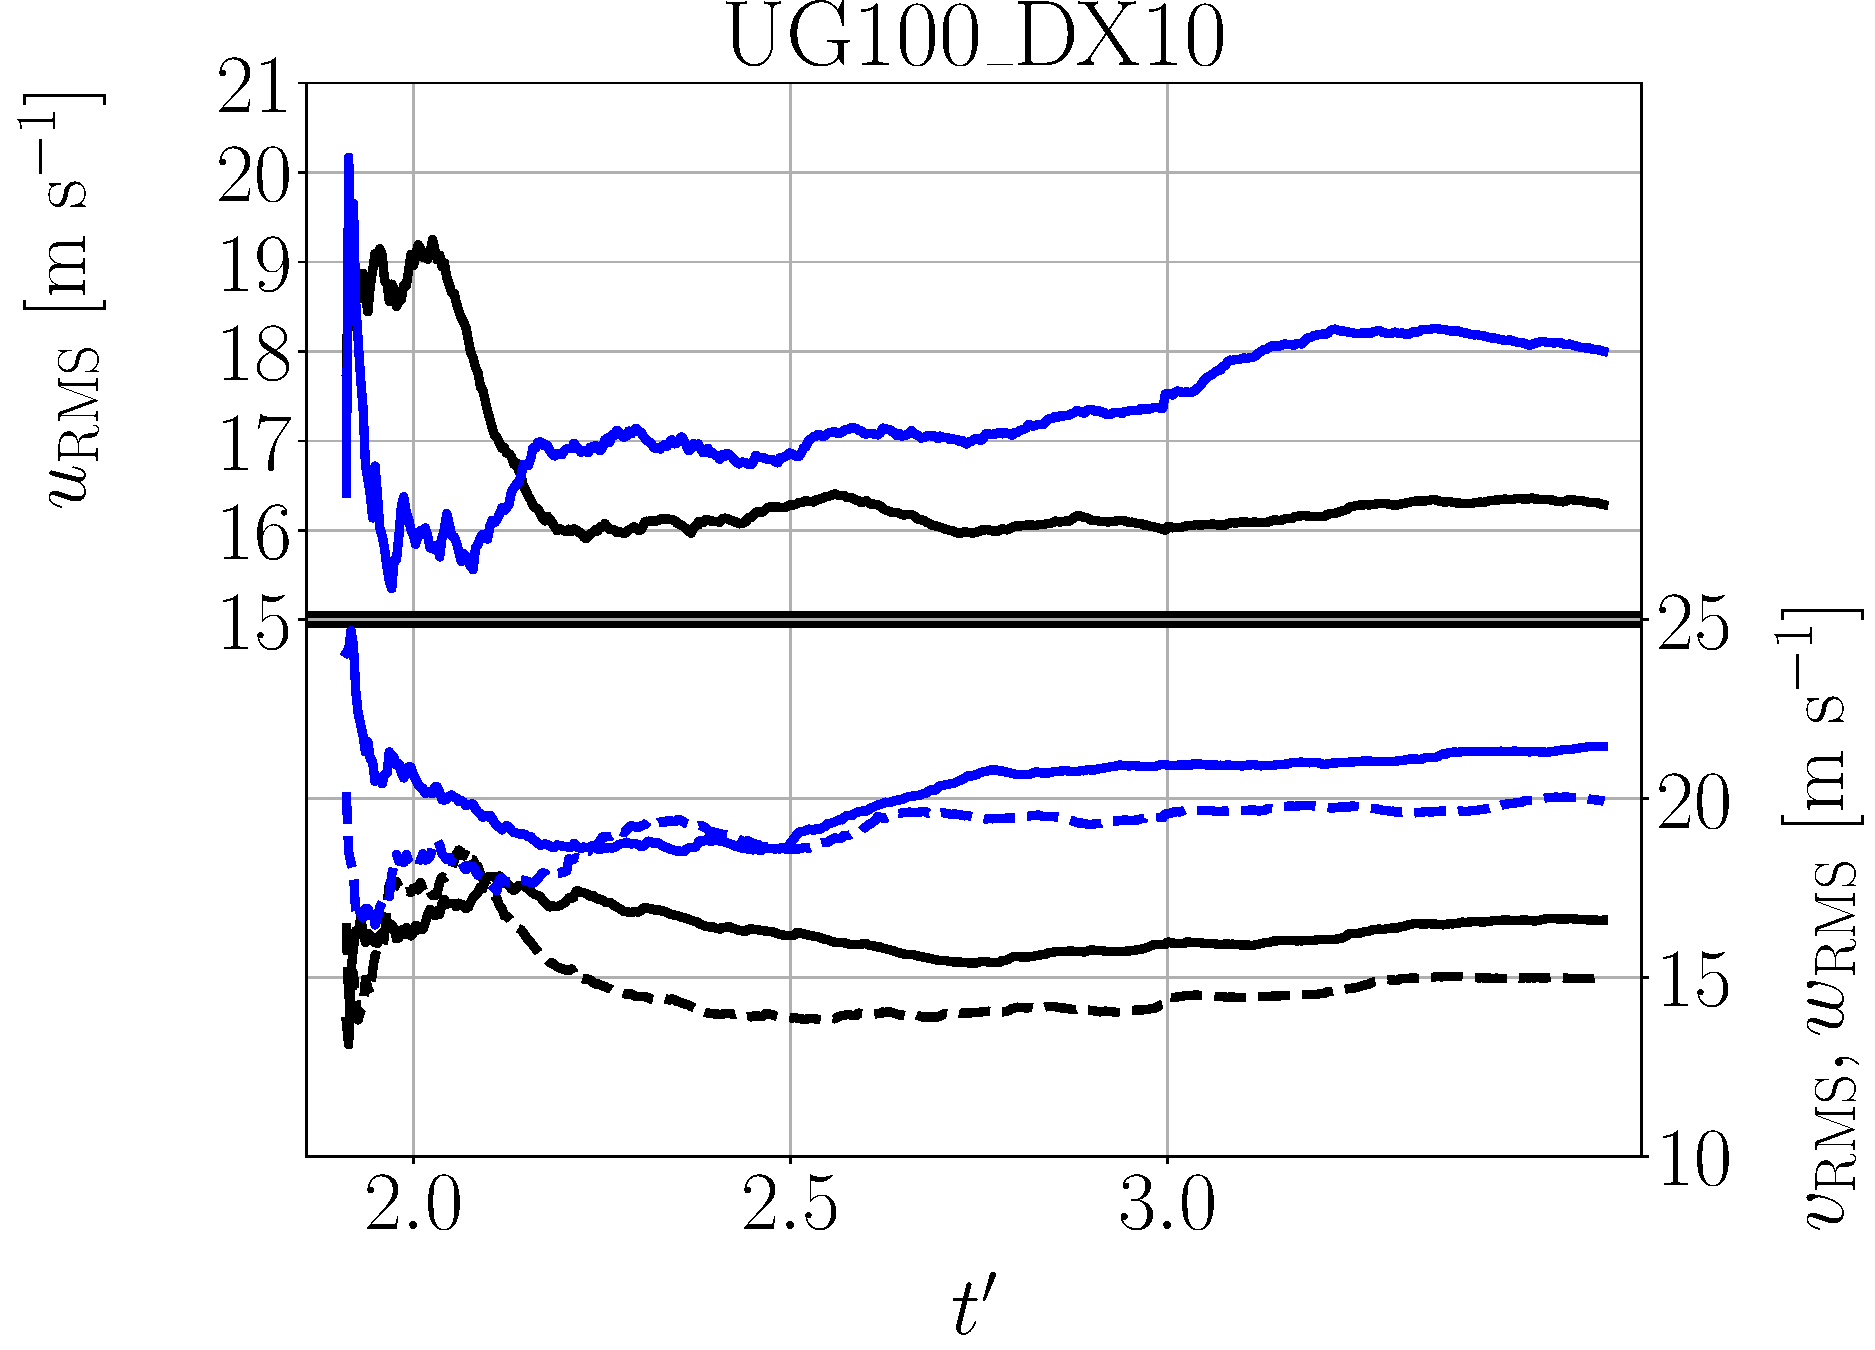
\includegraphics[width=0.3\textwidth]{./part2_developments/figures_ch5_resolved_JICF/SPRAY_characterization/velocities_establishment/establishment_UG100_DX10_rms}
   \hspace*{-0.1in}
   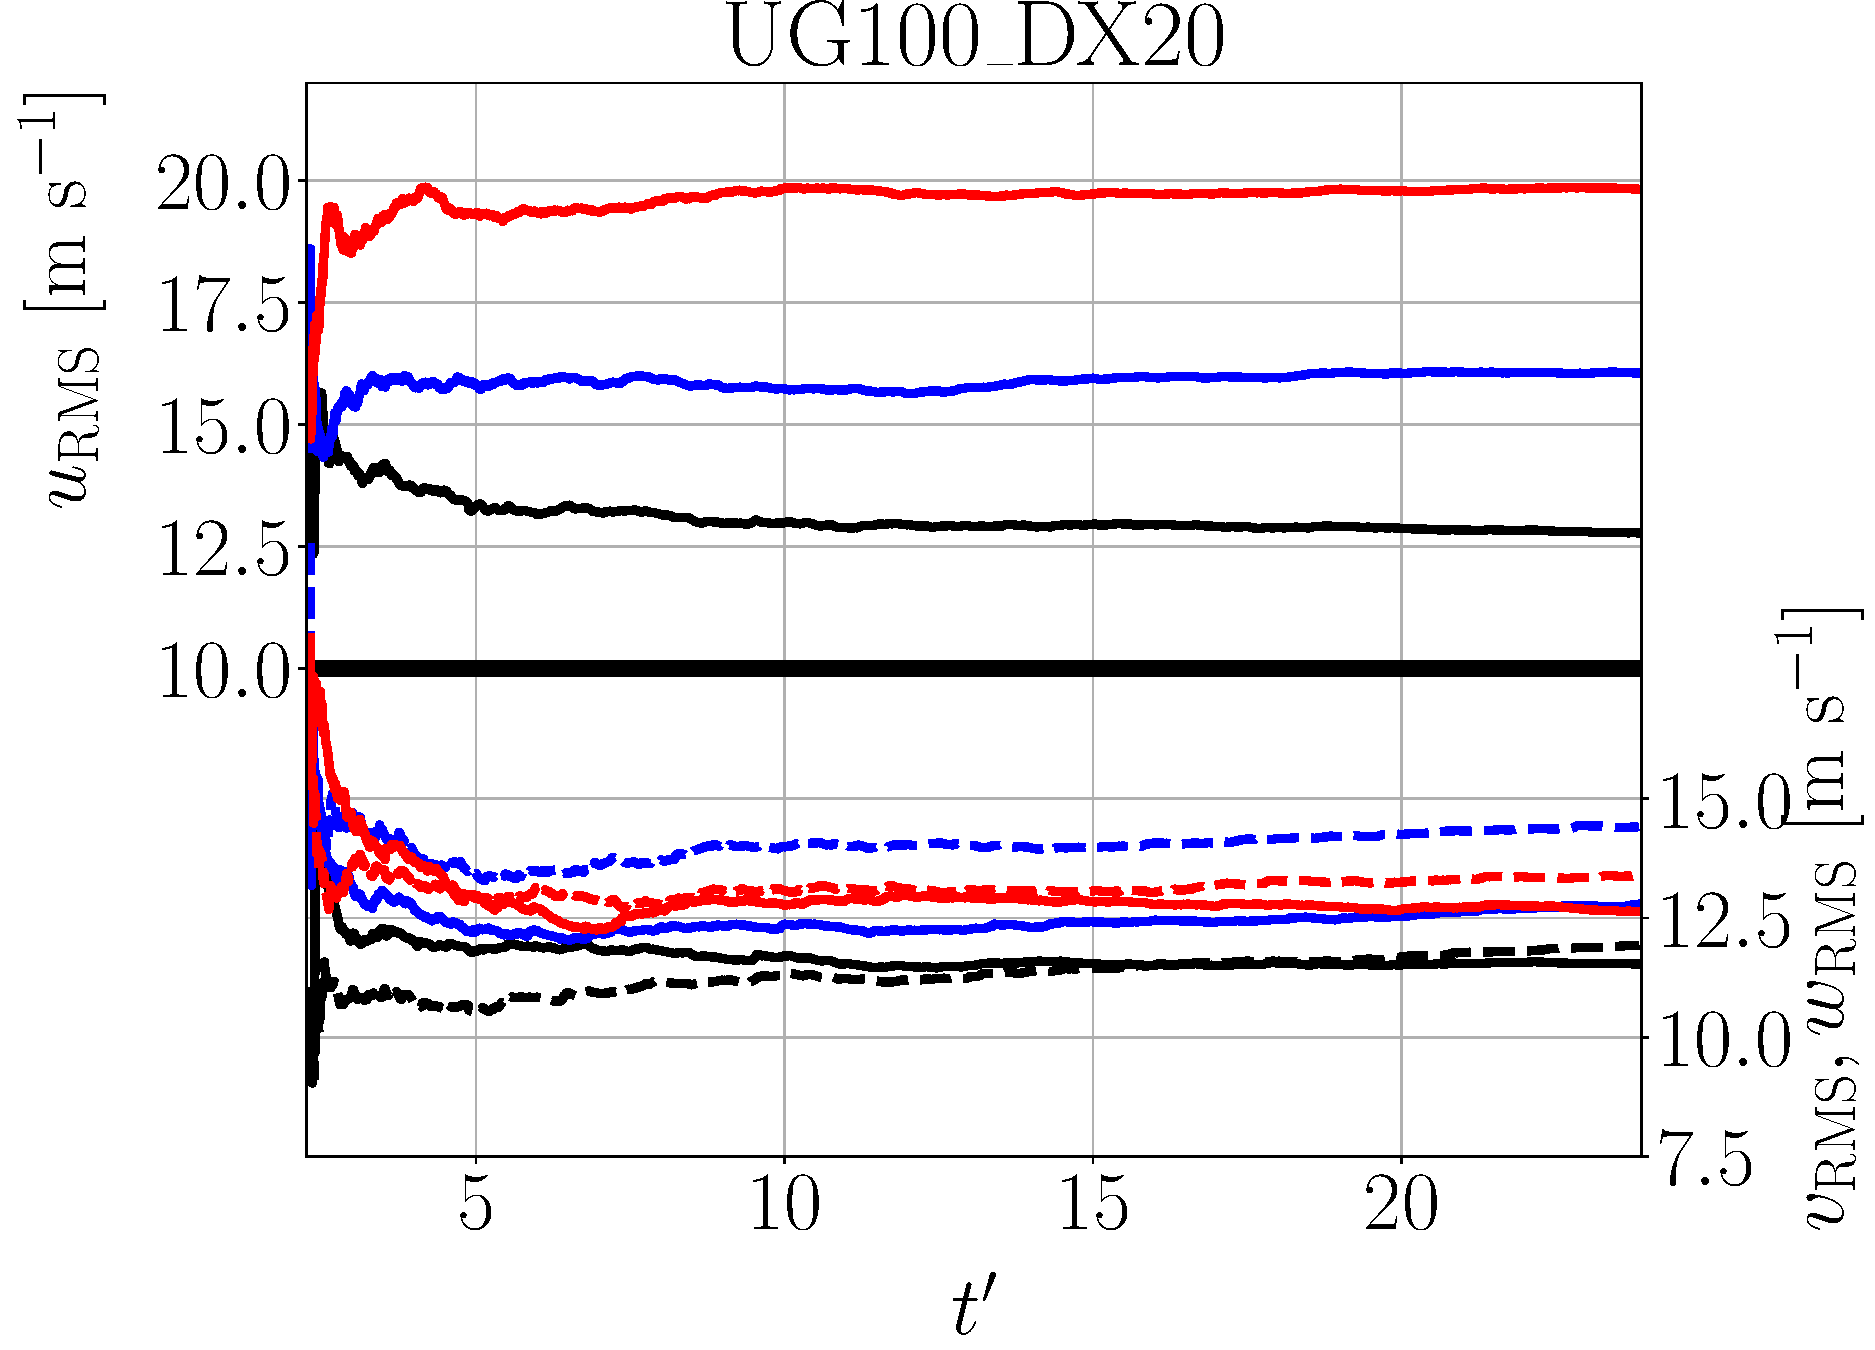
\includegraphics[width=0.3\textwidth]{./part2_developments/figures_ch5_resolved_JICF/SPRAY_characterization/velocities_establishment/establishment_UG100_DX20_rms}
   \hspace*{-0.1in}
   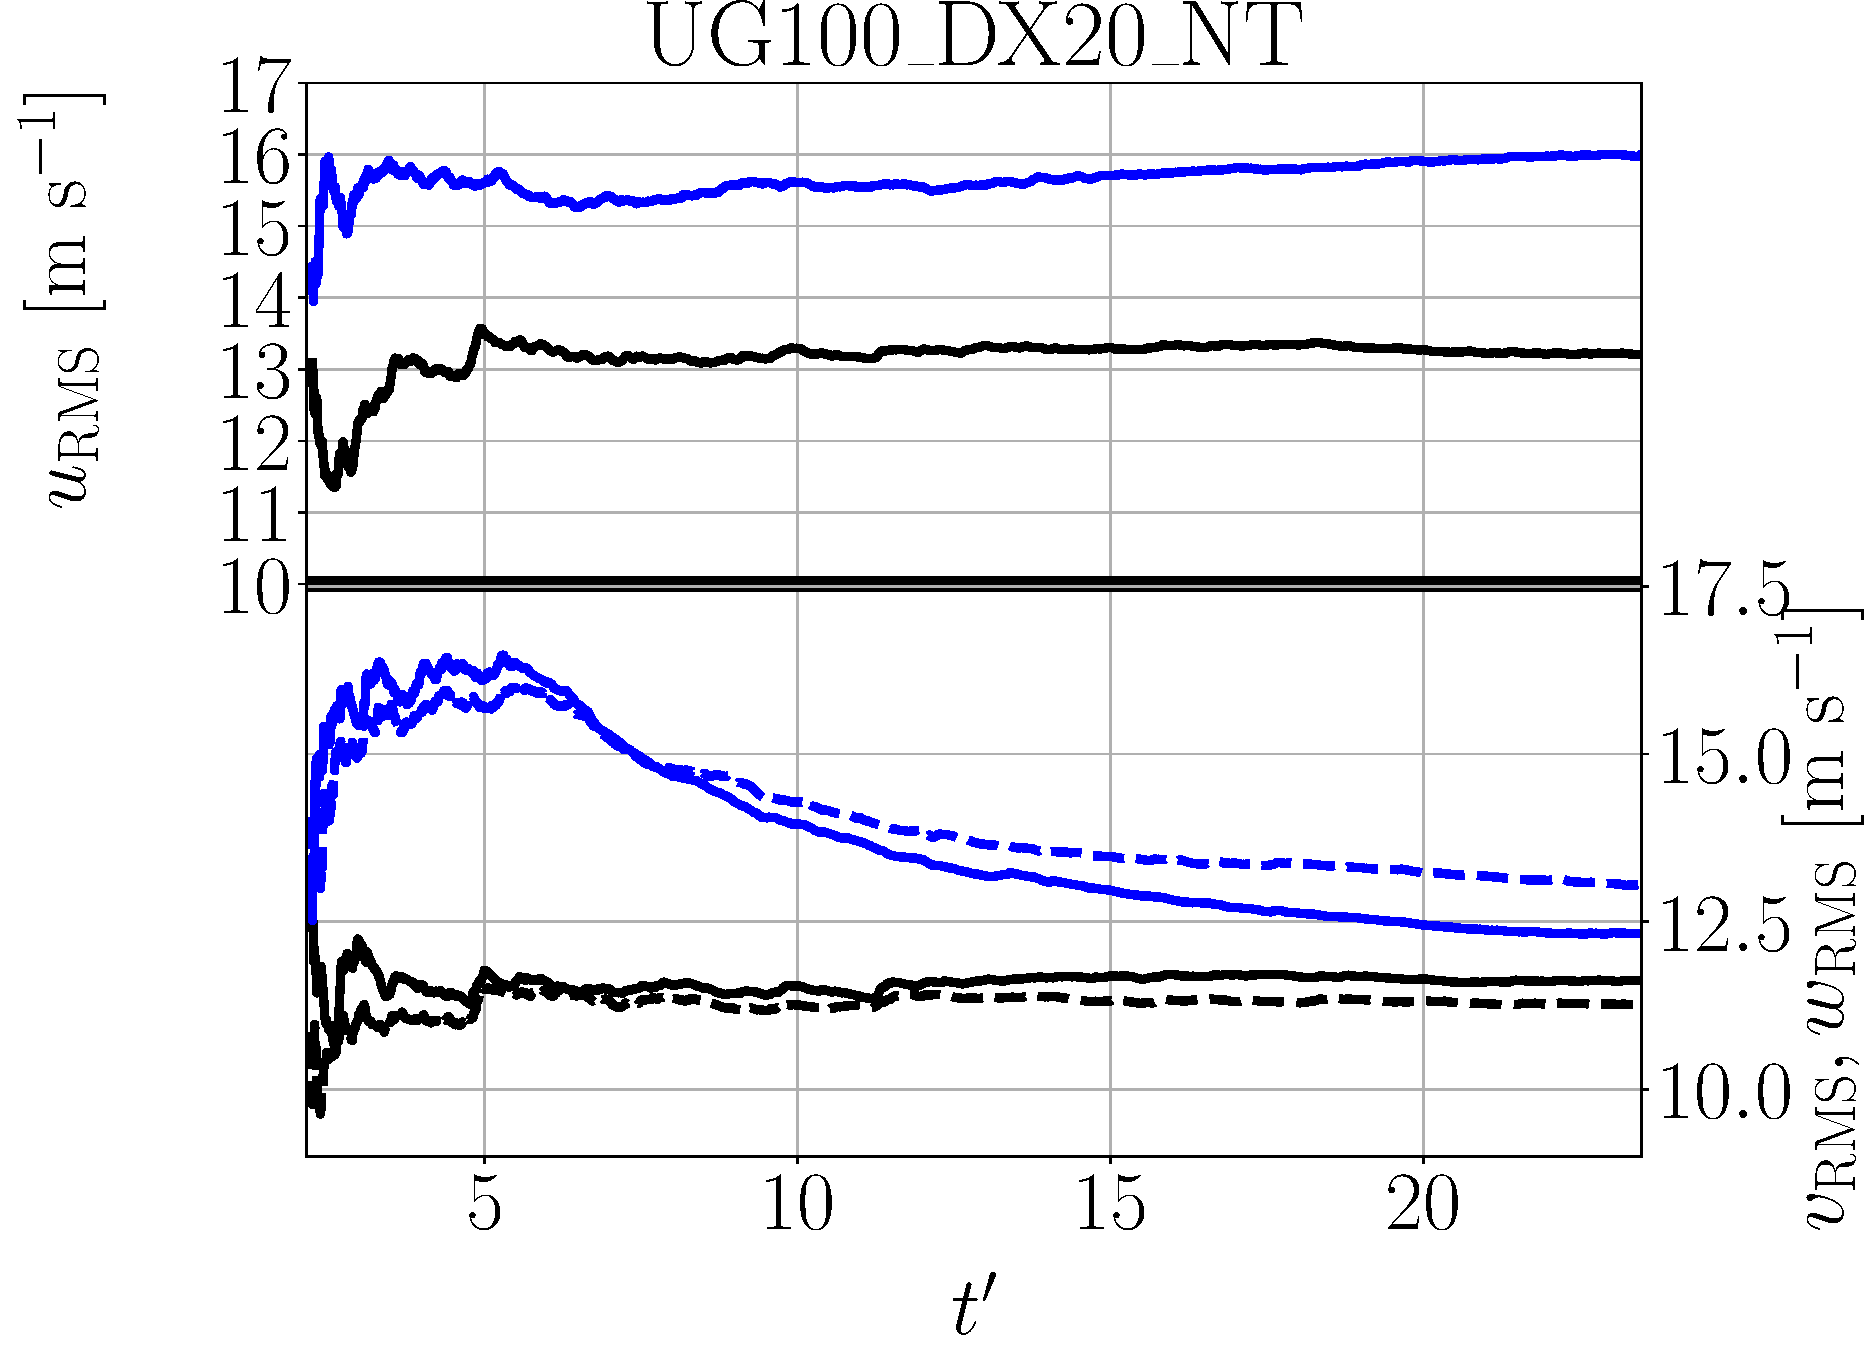
\includegraphics[width=0.3\textwidth]{./part2_developments/figures_ch5_resolved_JICF/SPRAY_characterization/velocities_establishment/establishment_UG100_DX20_NT_rms}
   \caption{Establishment of RMS liquid velocities for each case.}
\label{fig:app_spray_velocities_establishment_rms}
\end{figure}

\clearpage

\subsection*{Deformation parameters}

\begin{figure}[ht]
	\centering
   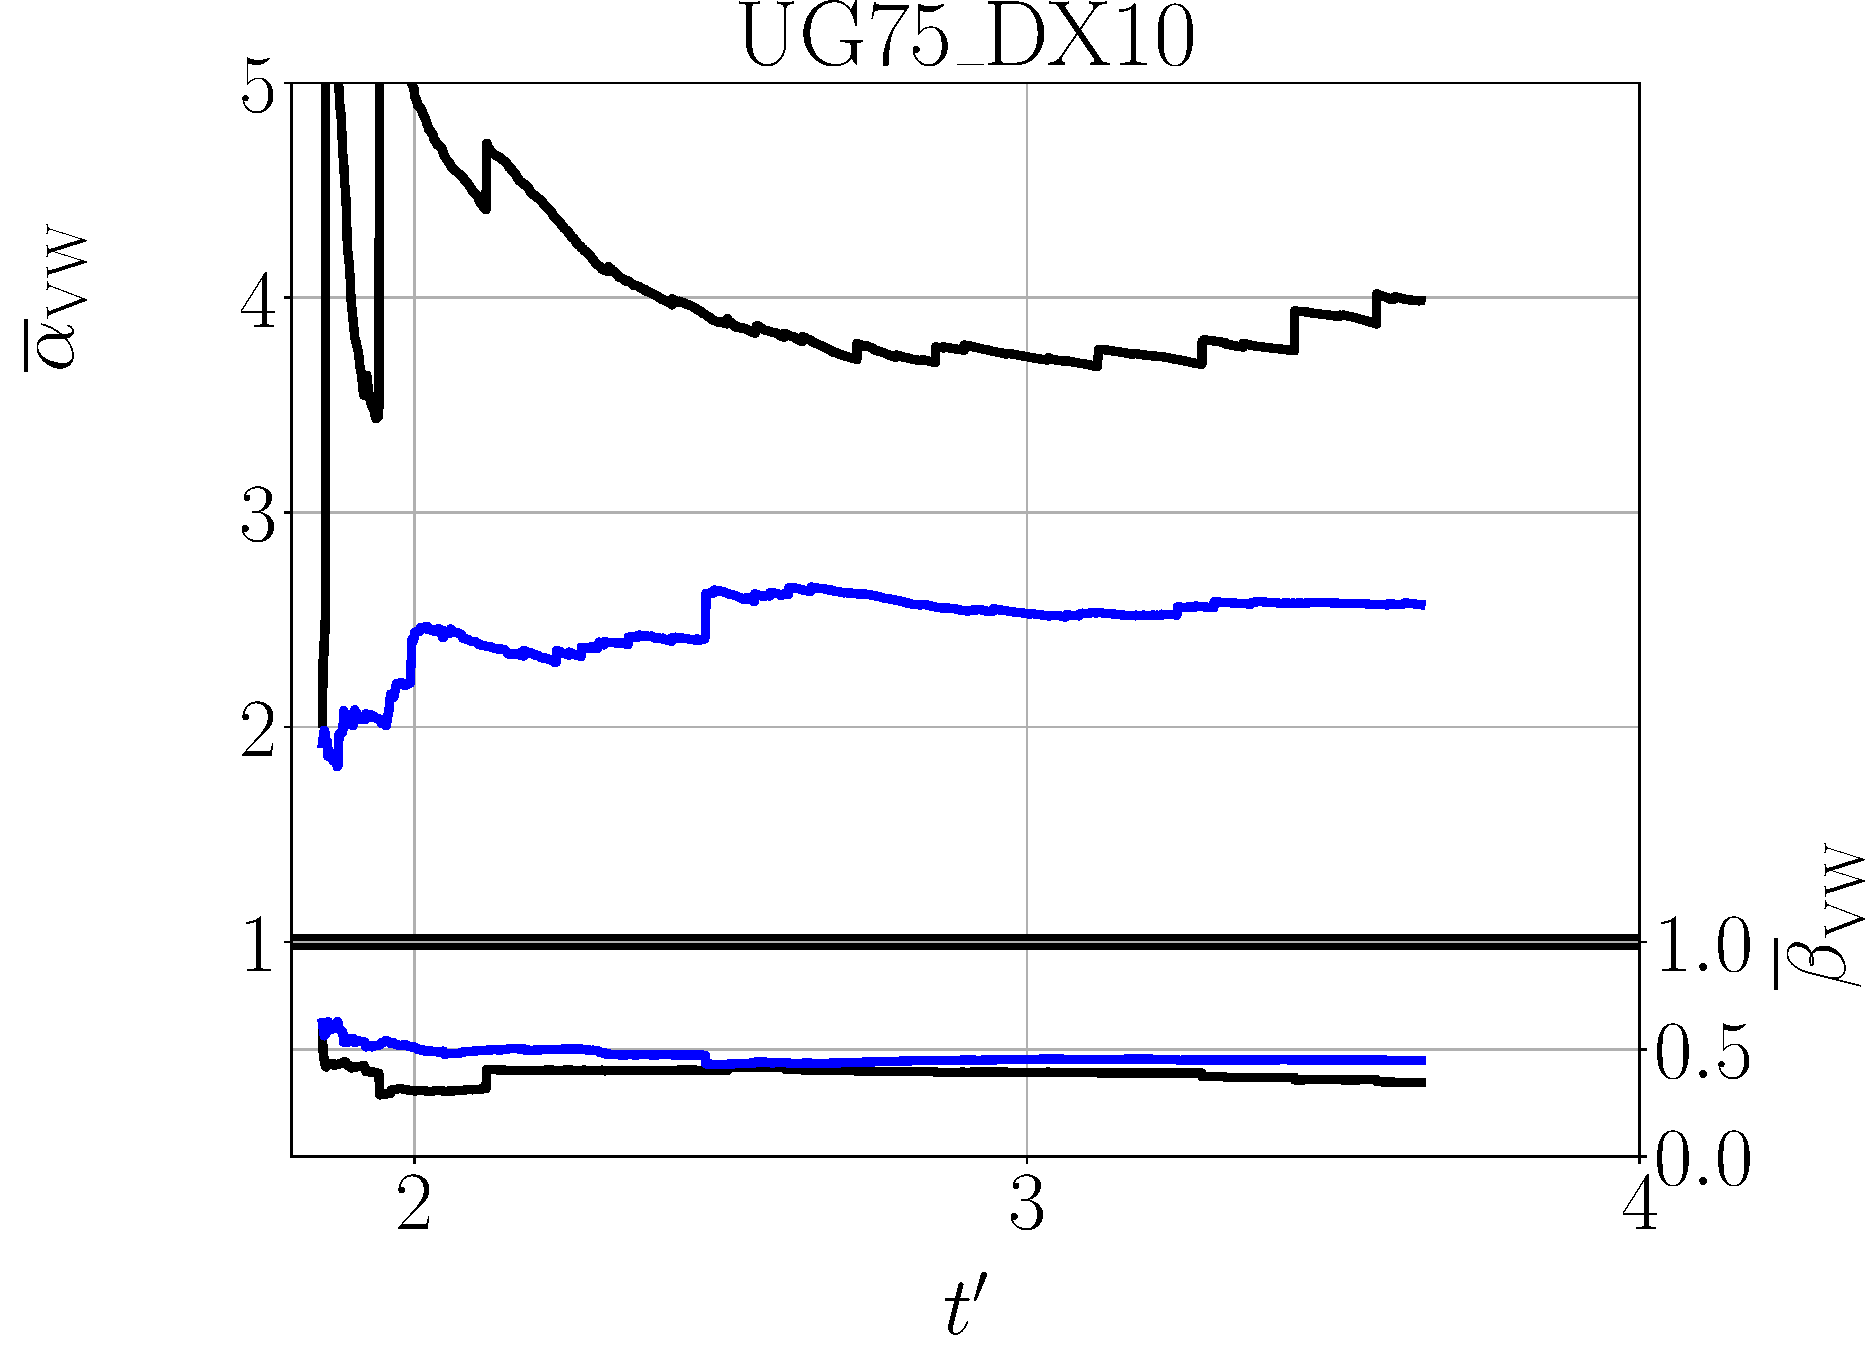
\includegraphics[width=0.3\textwidth]{./part2_developments/figures_ch5_resolved_JICF/SPRAY_characterization/deformation_establishment/establishment_UG75_DX10_mean}
   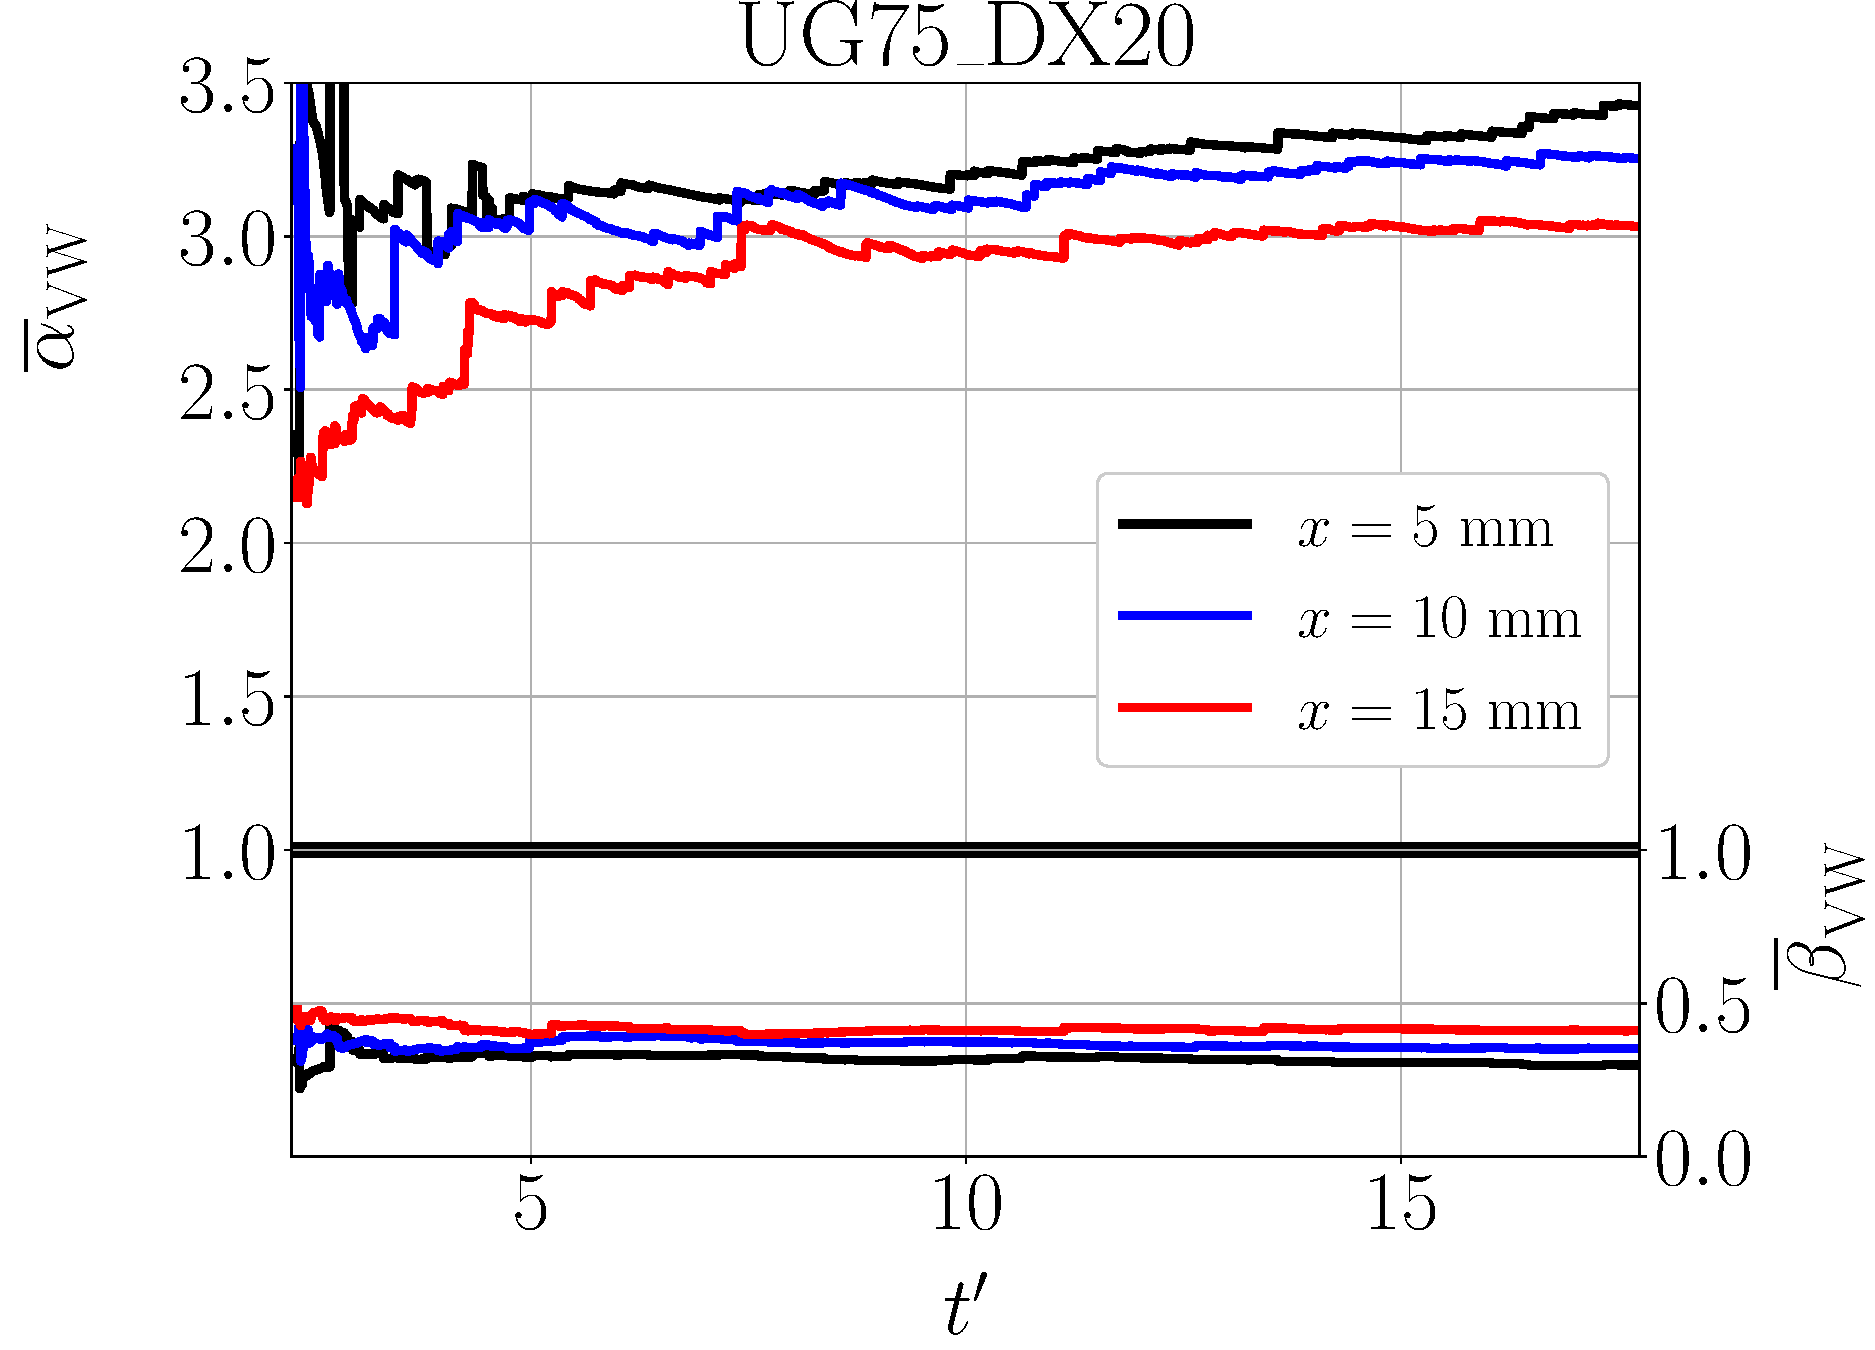
\includegraphics[width=0.3\textwidth]{./part2_developments/figures_ch5_resolved_JICF/SPRAY_characterization/deformation_establishment/establishment_UG75_DX20_mean}
   
	\vskip\baselineskip
	
   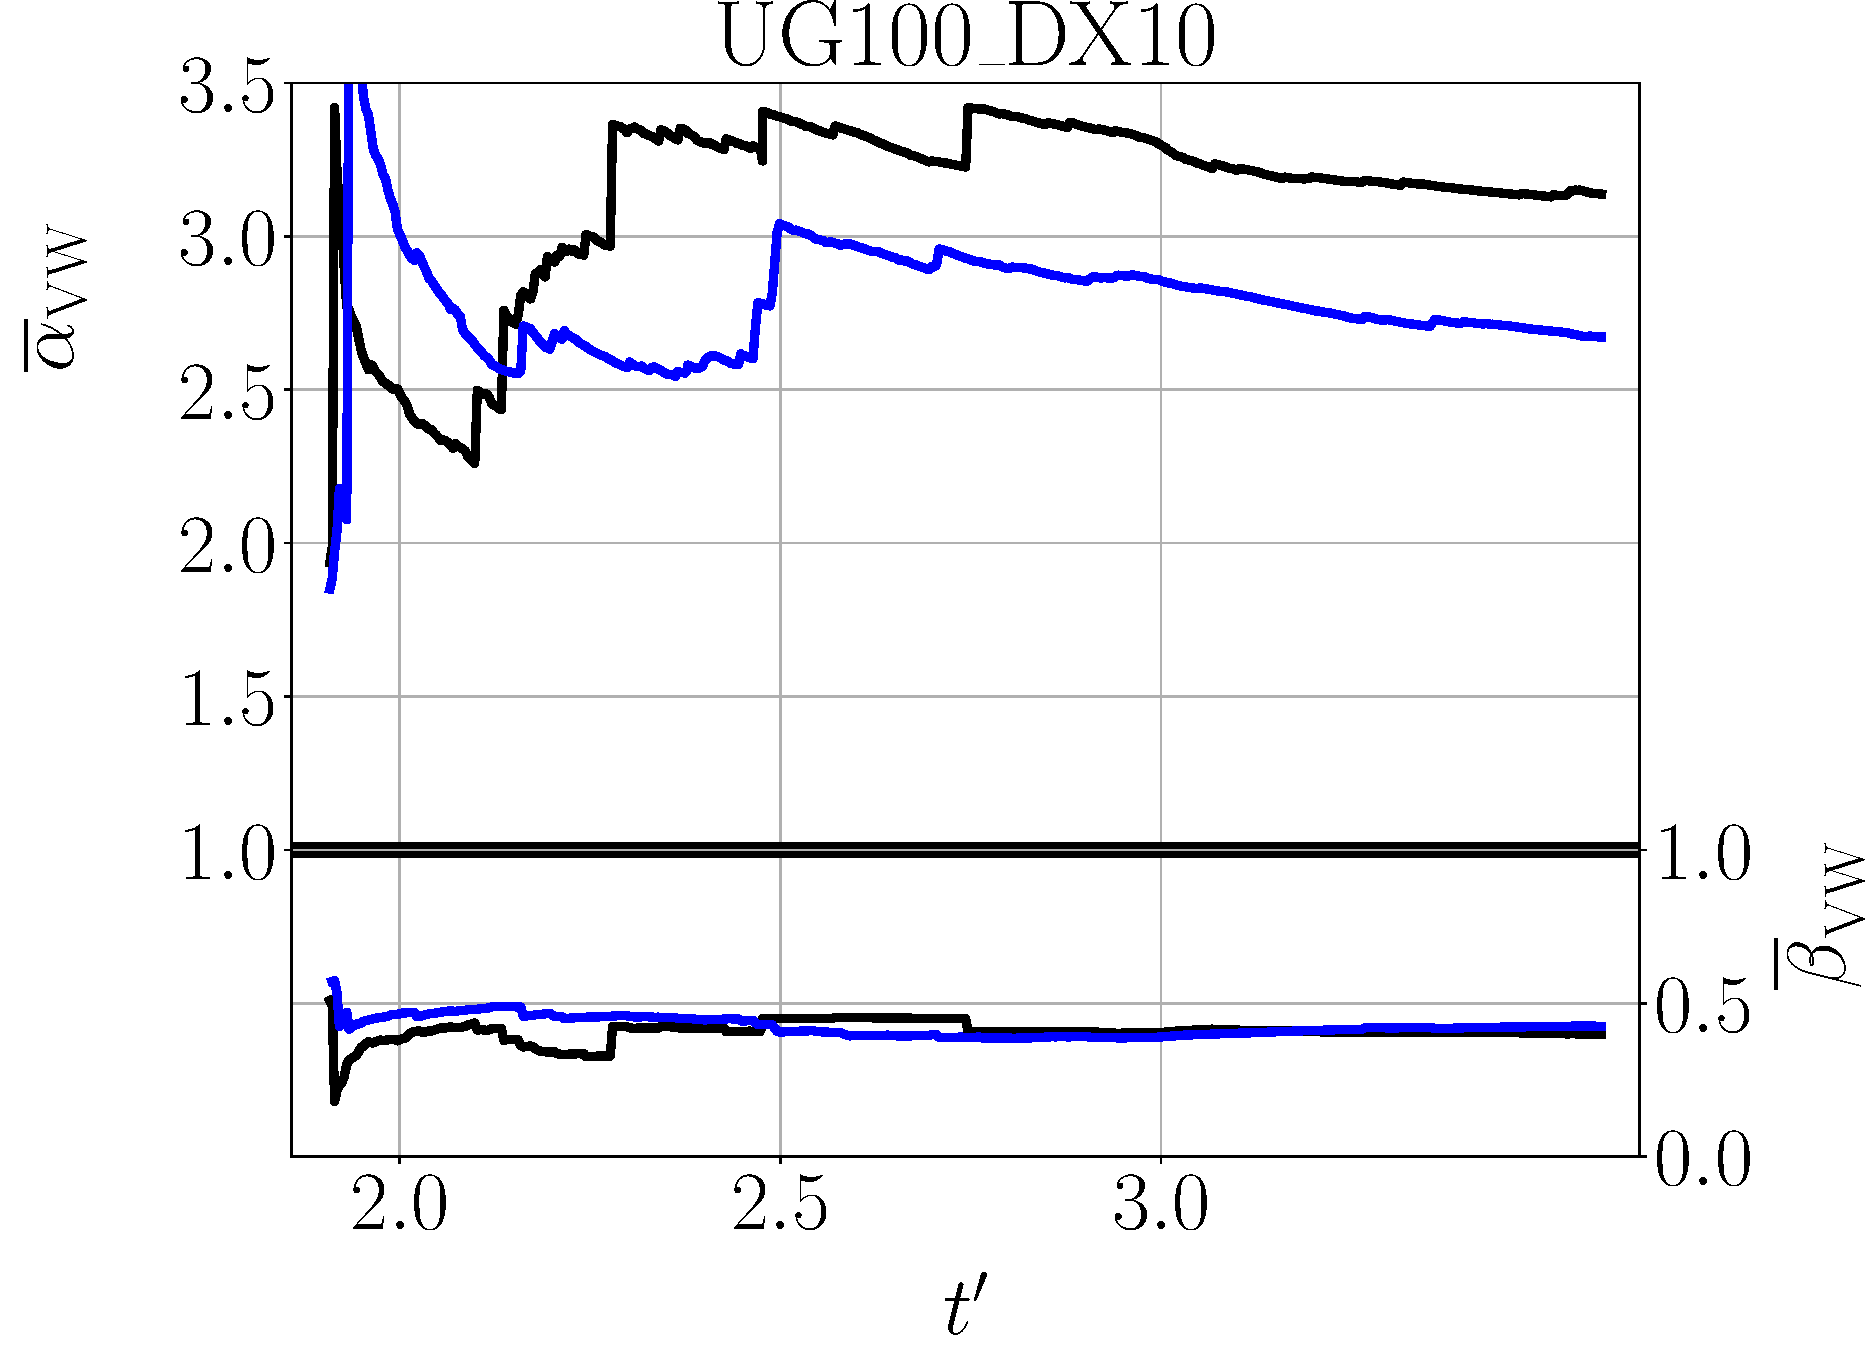
\includegraphics[width=0.3\textwidth]{./part2_developments/figures_ch5_resolved_JICF/SPRAY_characterization/deformation_establishment/establishment_UG100_DX10_mean}
   \hspace*{-0.1in}
   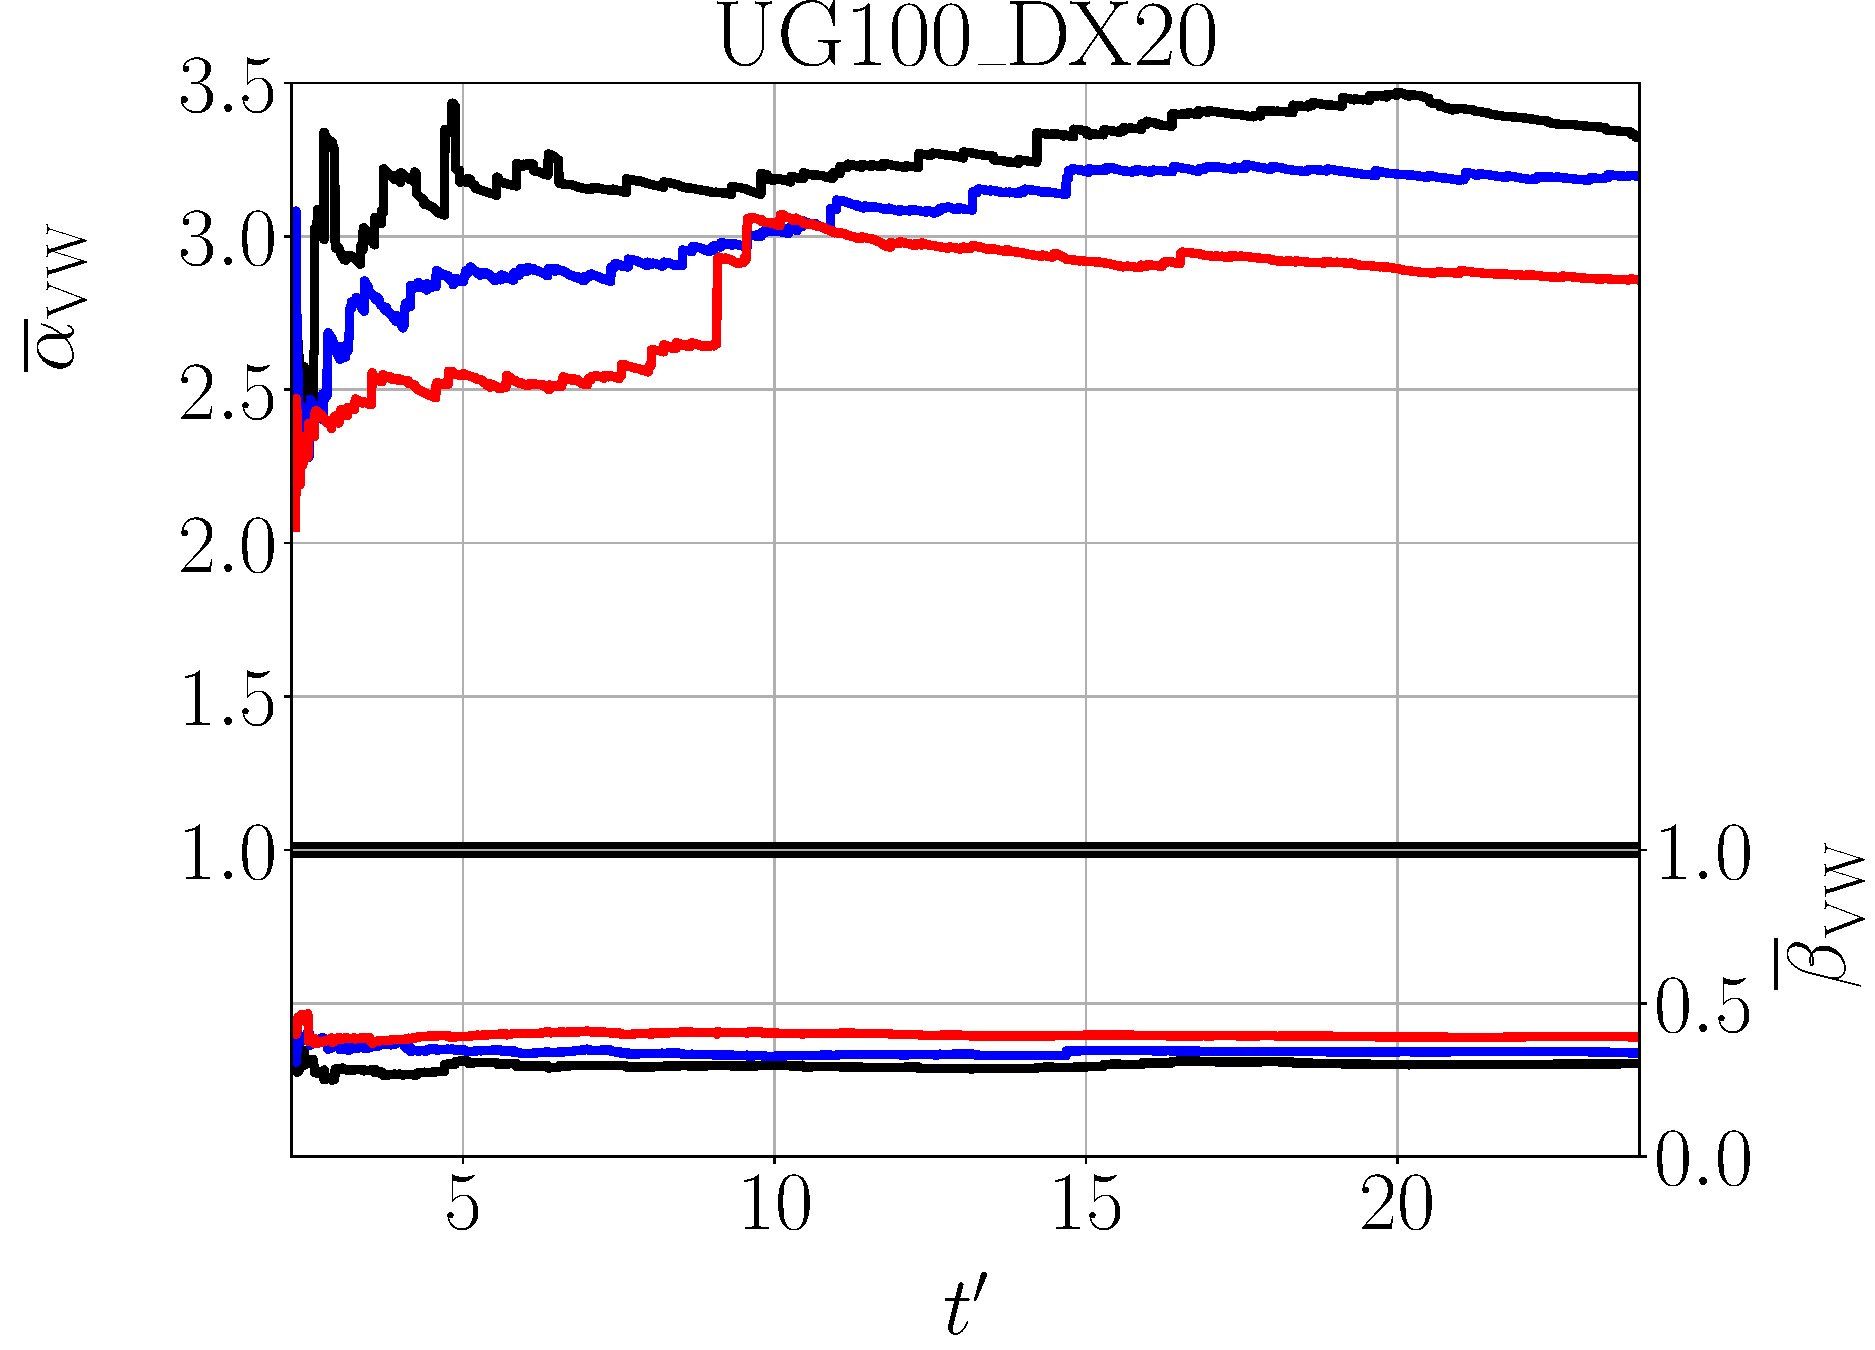
\includegraphics[width=0.3\textwidth]{./part2_developments/figures_ch5_resolved_JICF/SPRAY_characterization/deformation_establishment/establishment_UG100_DX20_mean}
   \hspace*{-0.1in}
   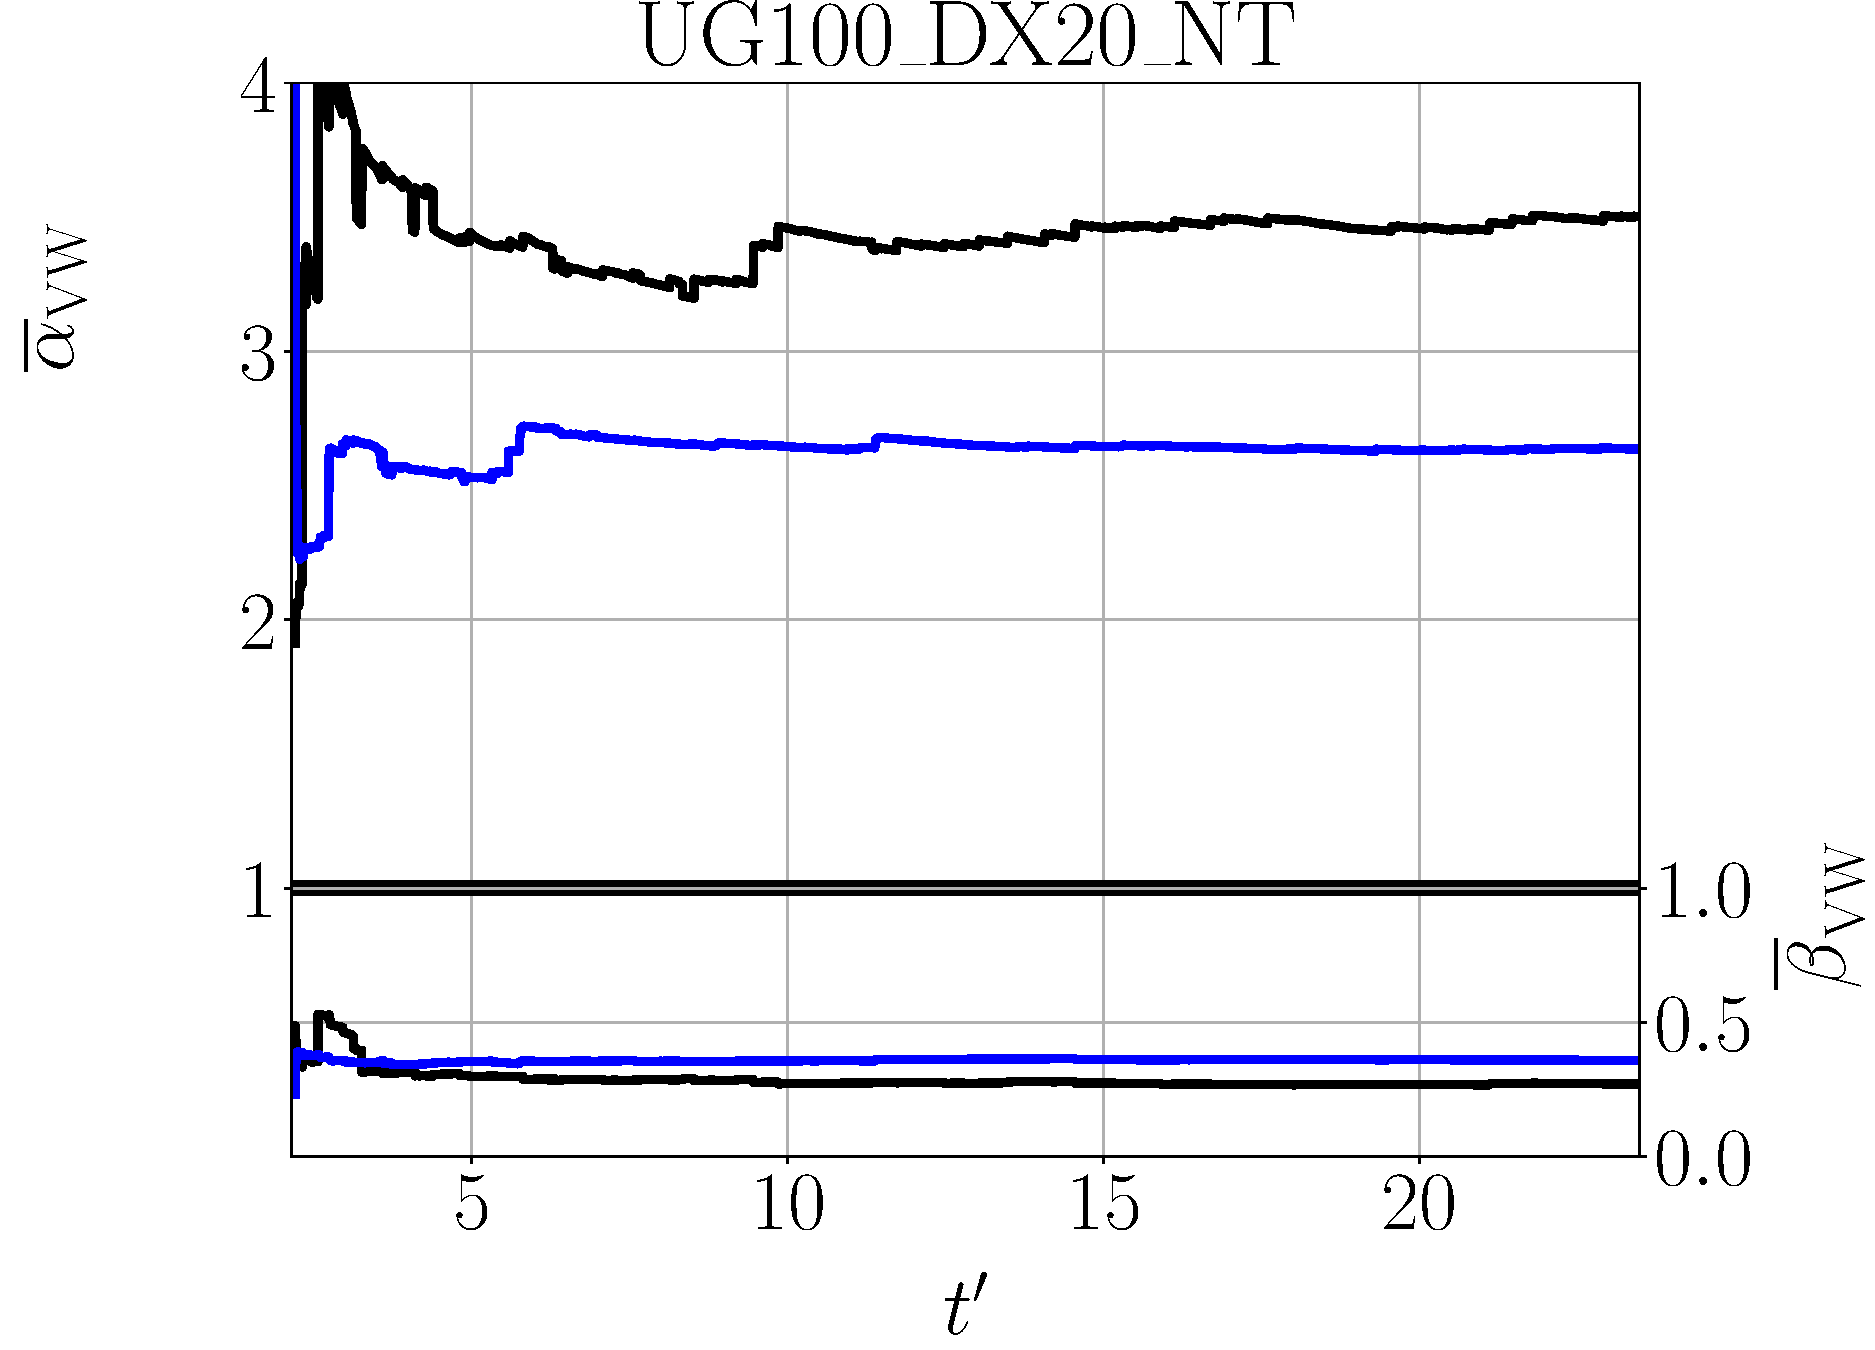
\includegraphics[width=0.3\textwidth]{./part2_developments/figures_ch5_resolved_JICF/SPRAY_characterization/deformation_establishment/establishment_UG100_DX20_NT_mean}
   \caption{Establishment of mean deformation parameters for each case.}
\label{fig:app_spray_deformation_establishment_mean}
\end{figure}

\vspace*{0.2in}

\begin{figure}[ht]
	\centering
   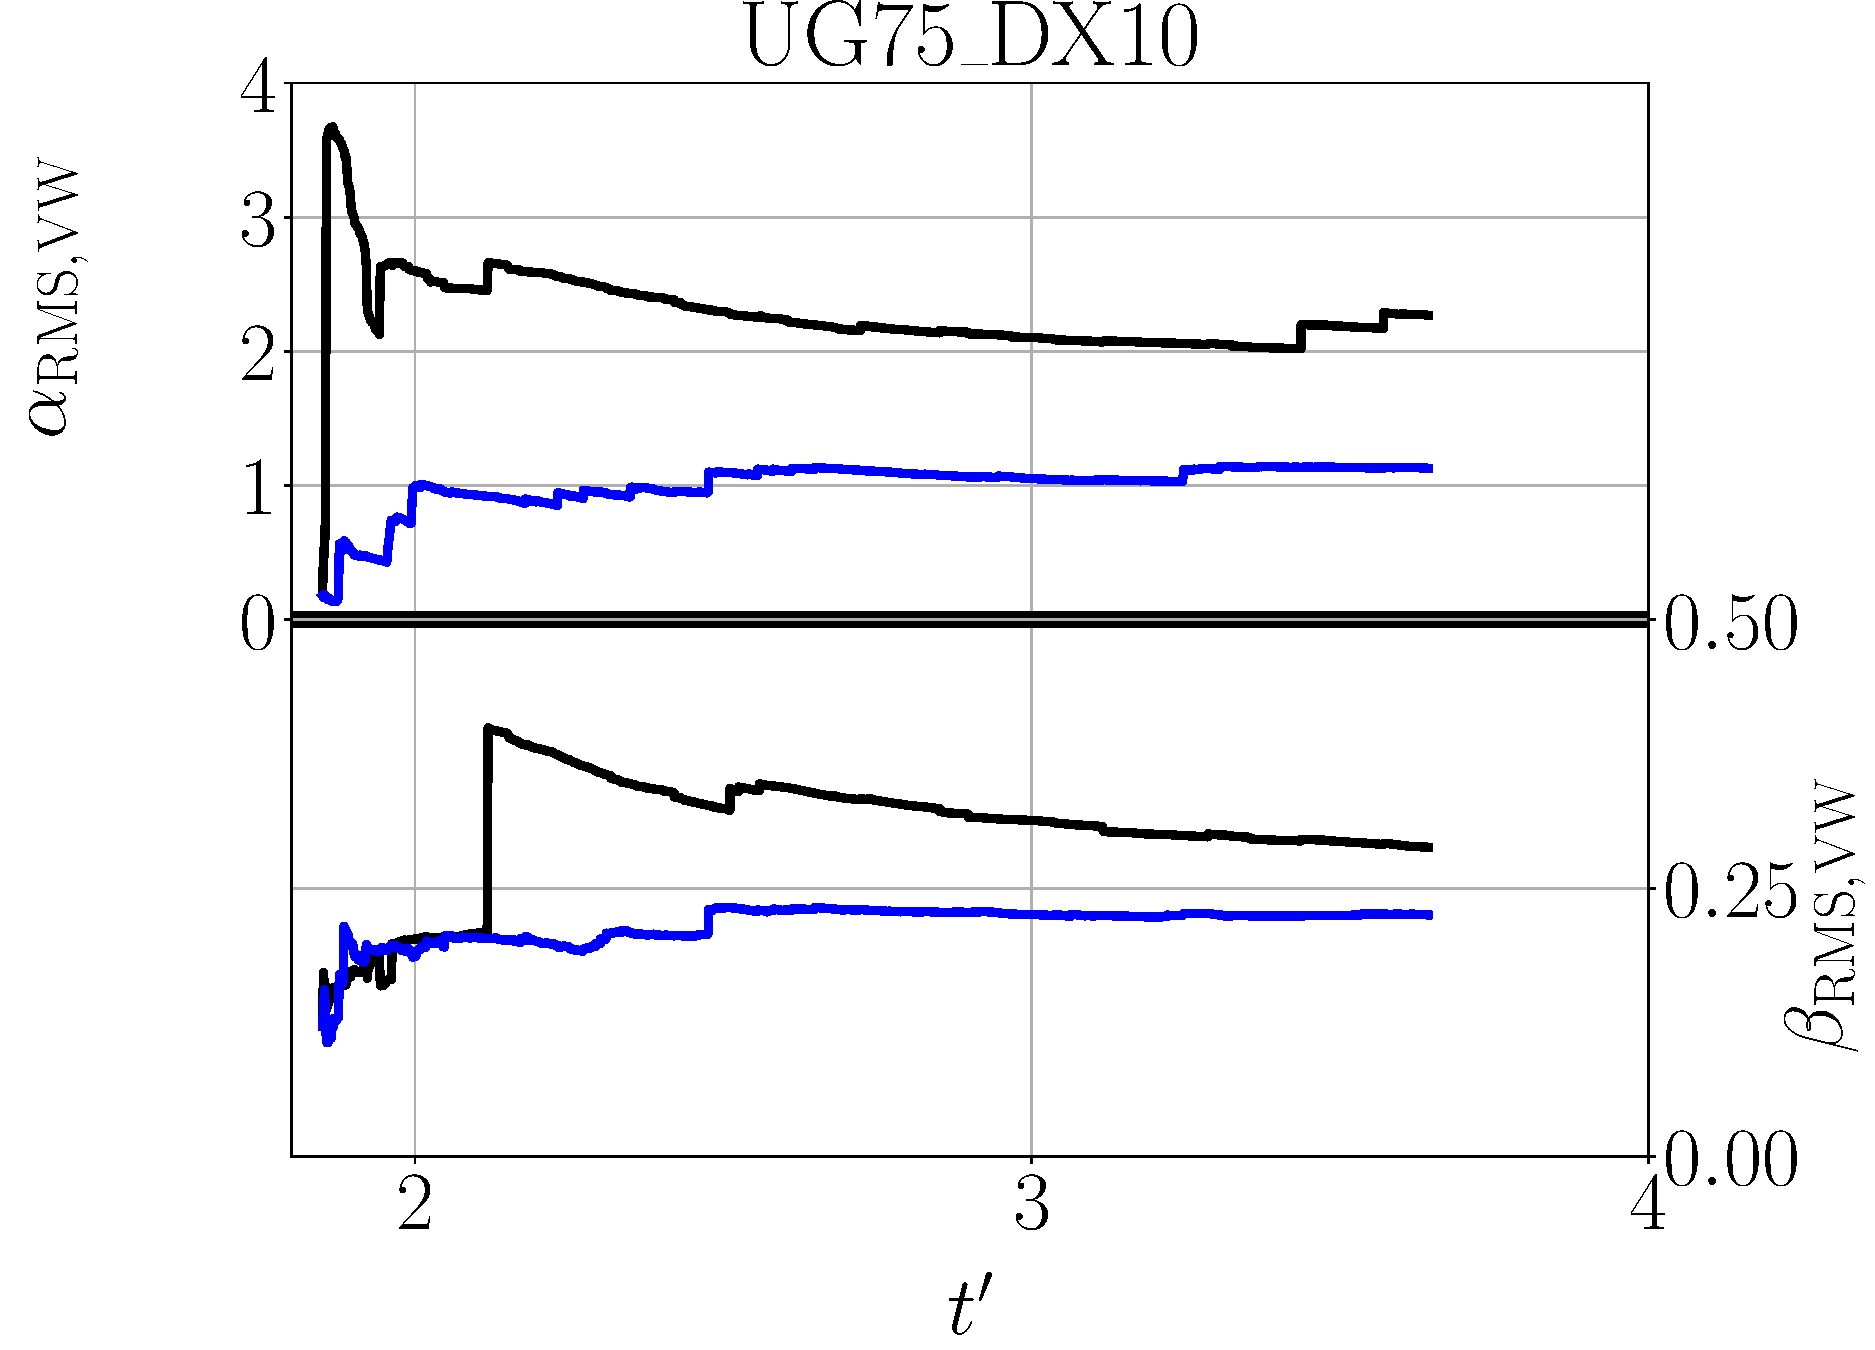
\includegraphics[width=0.3\textwidth]{./part2_developments/figures_ch5_resolved_JICF/SPRAY_characterization/deformation_establishment/establishment_UG75_DX10_rms}
   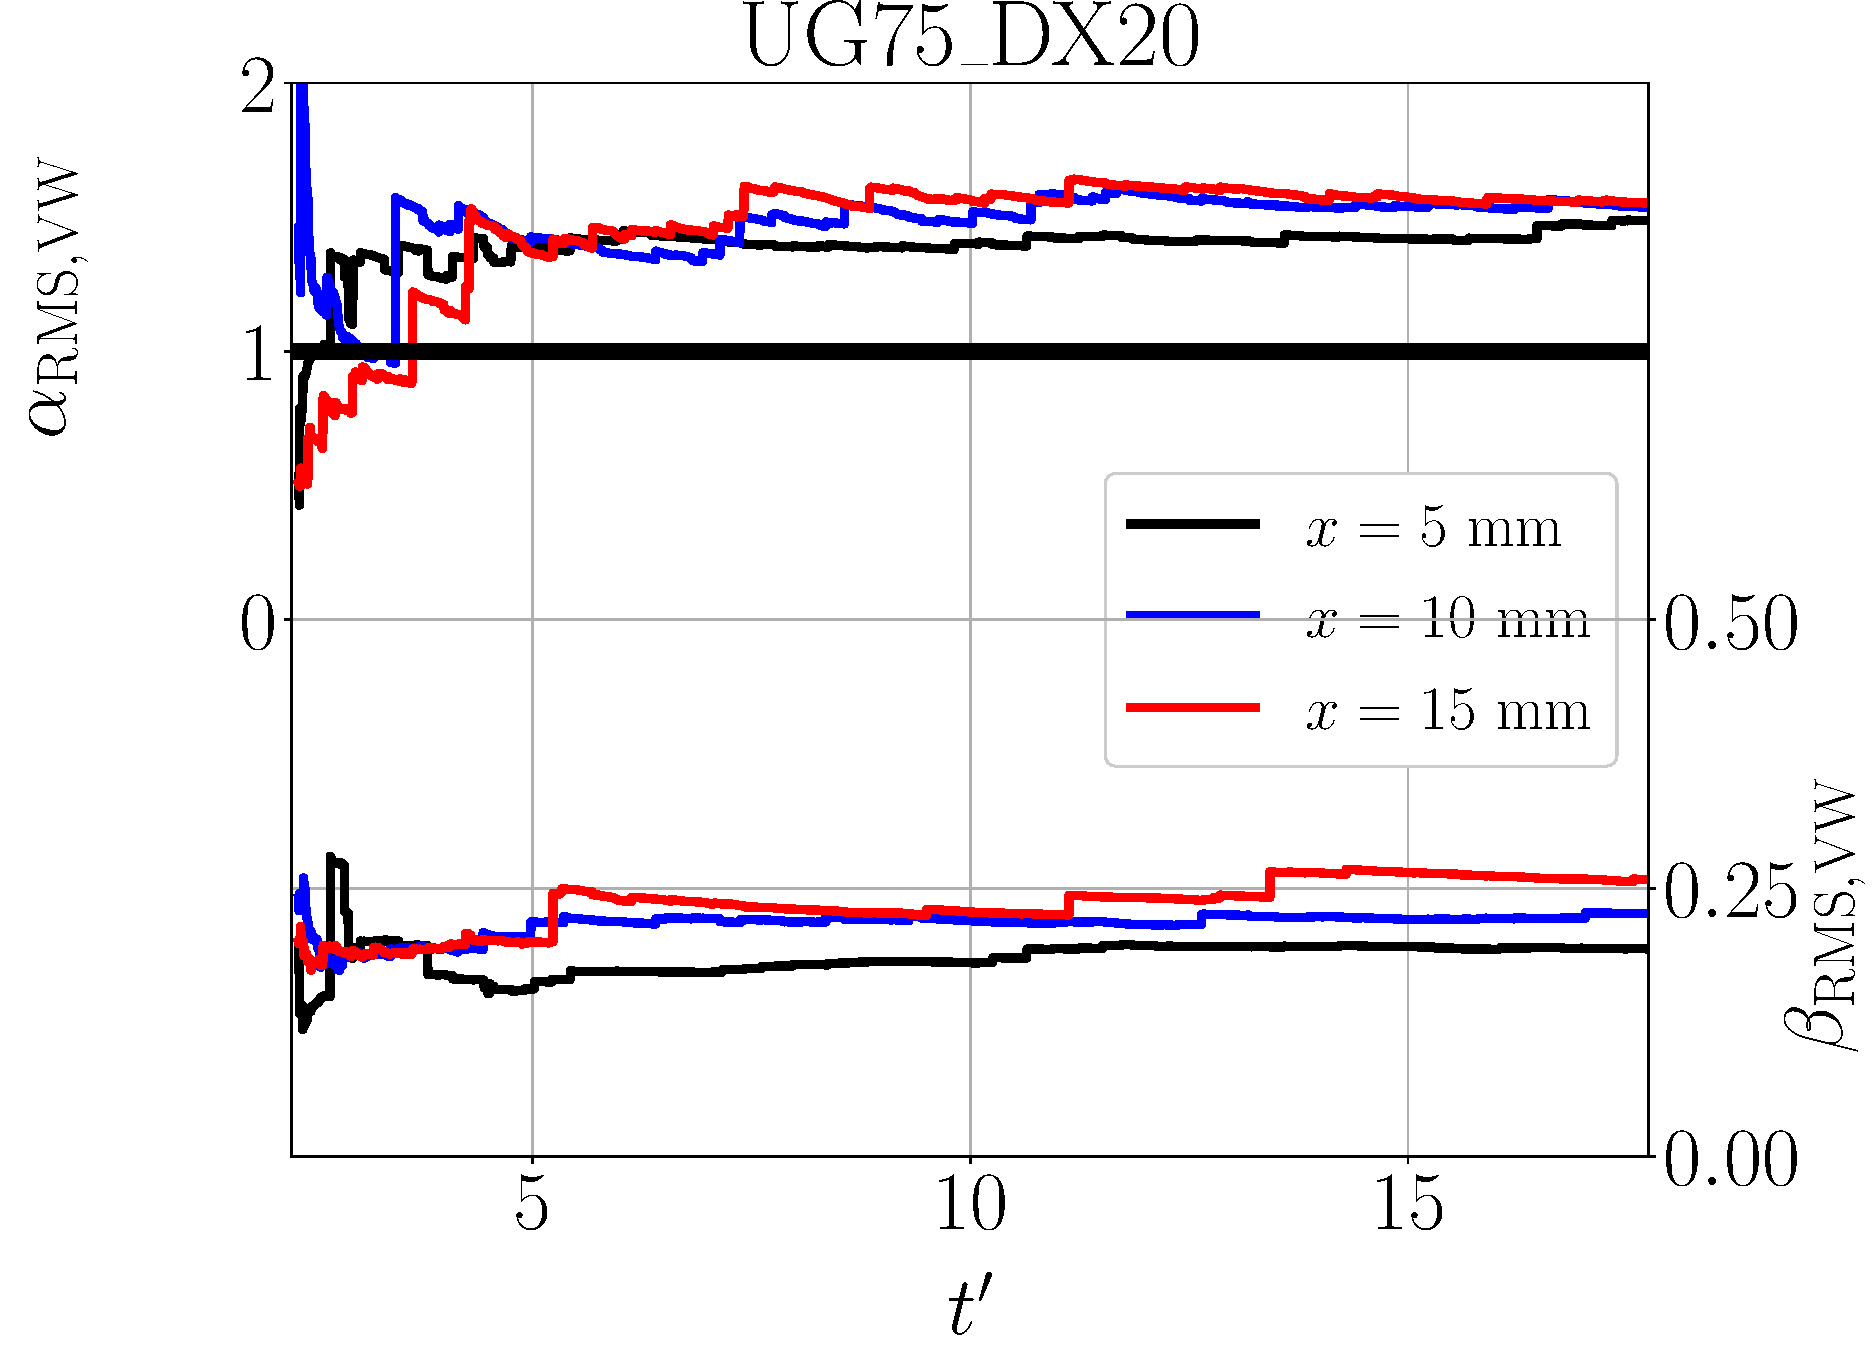
\includegraphics[width=0.3\textwidth]{./part2_developments/figures_ch5_resolved_JICF/SPRAY_characterization/deformation_establishment/establishment_UG75_DX20_rms}
   
	\vskip\baselineskip
	
   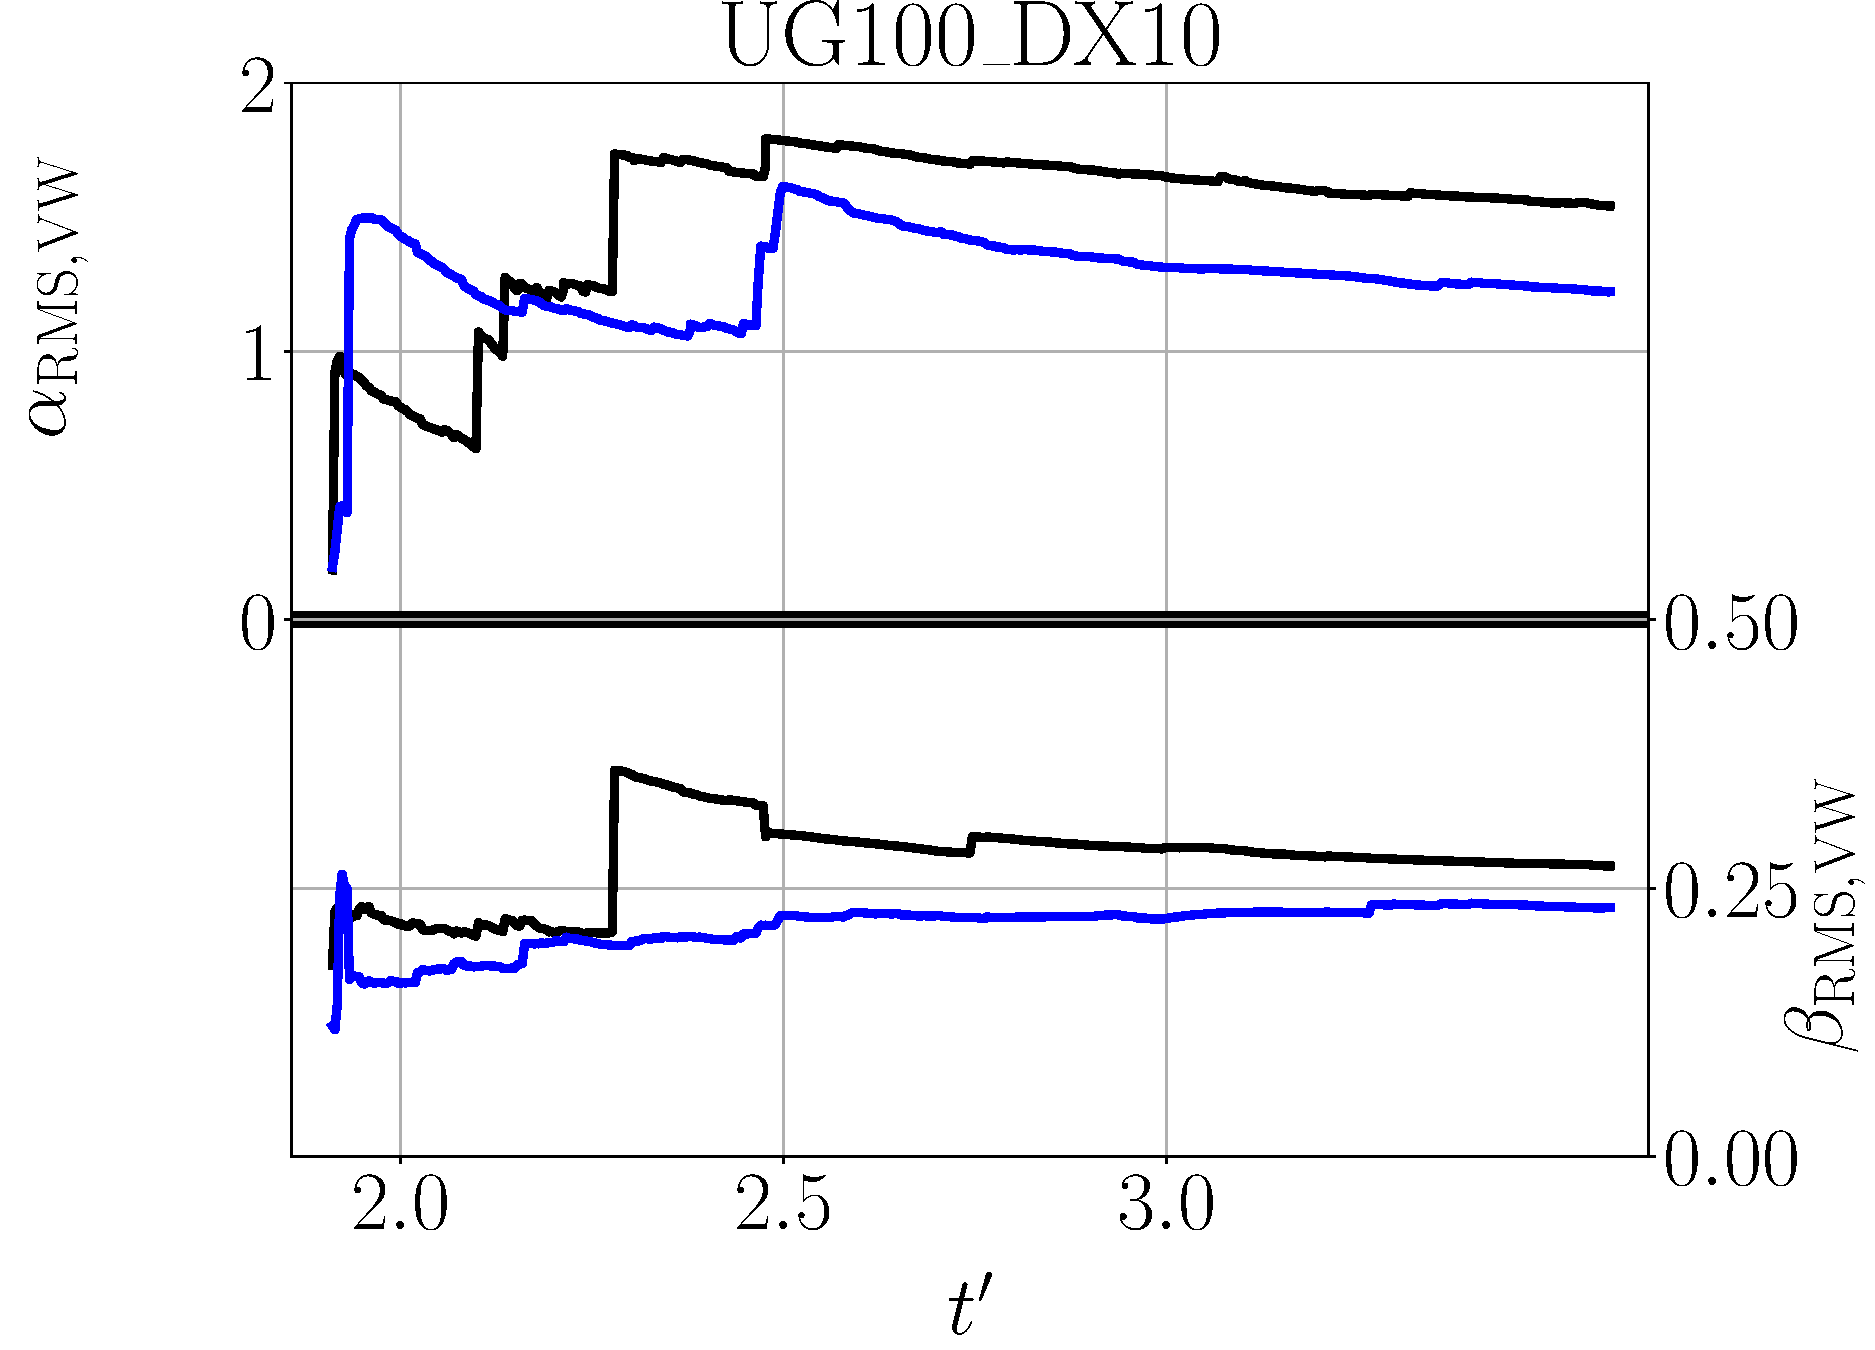
\includegraphics[width=0.3\textwidth]{./part2_developments/figures_ch5_resolved_JICF/SPRAY_characterization/deformation_establishment/establishment_UG100_DX10_rms}
   \hspace*{-0.1in}
   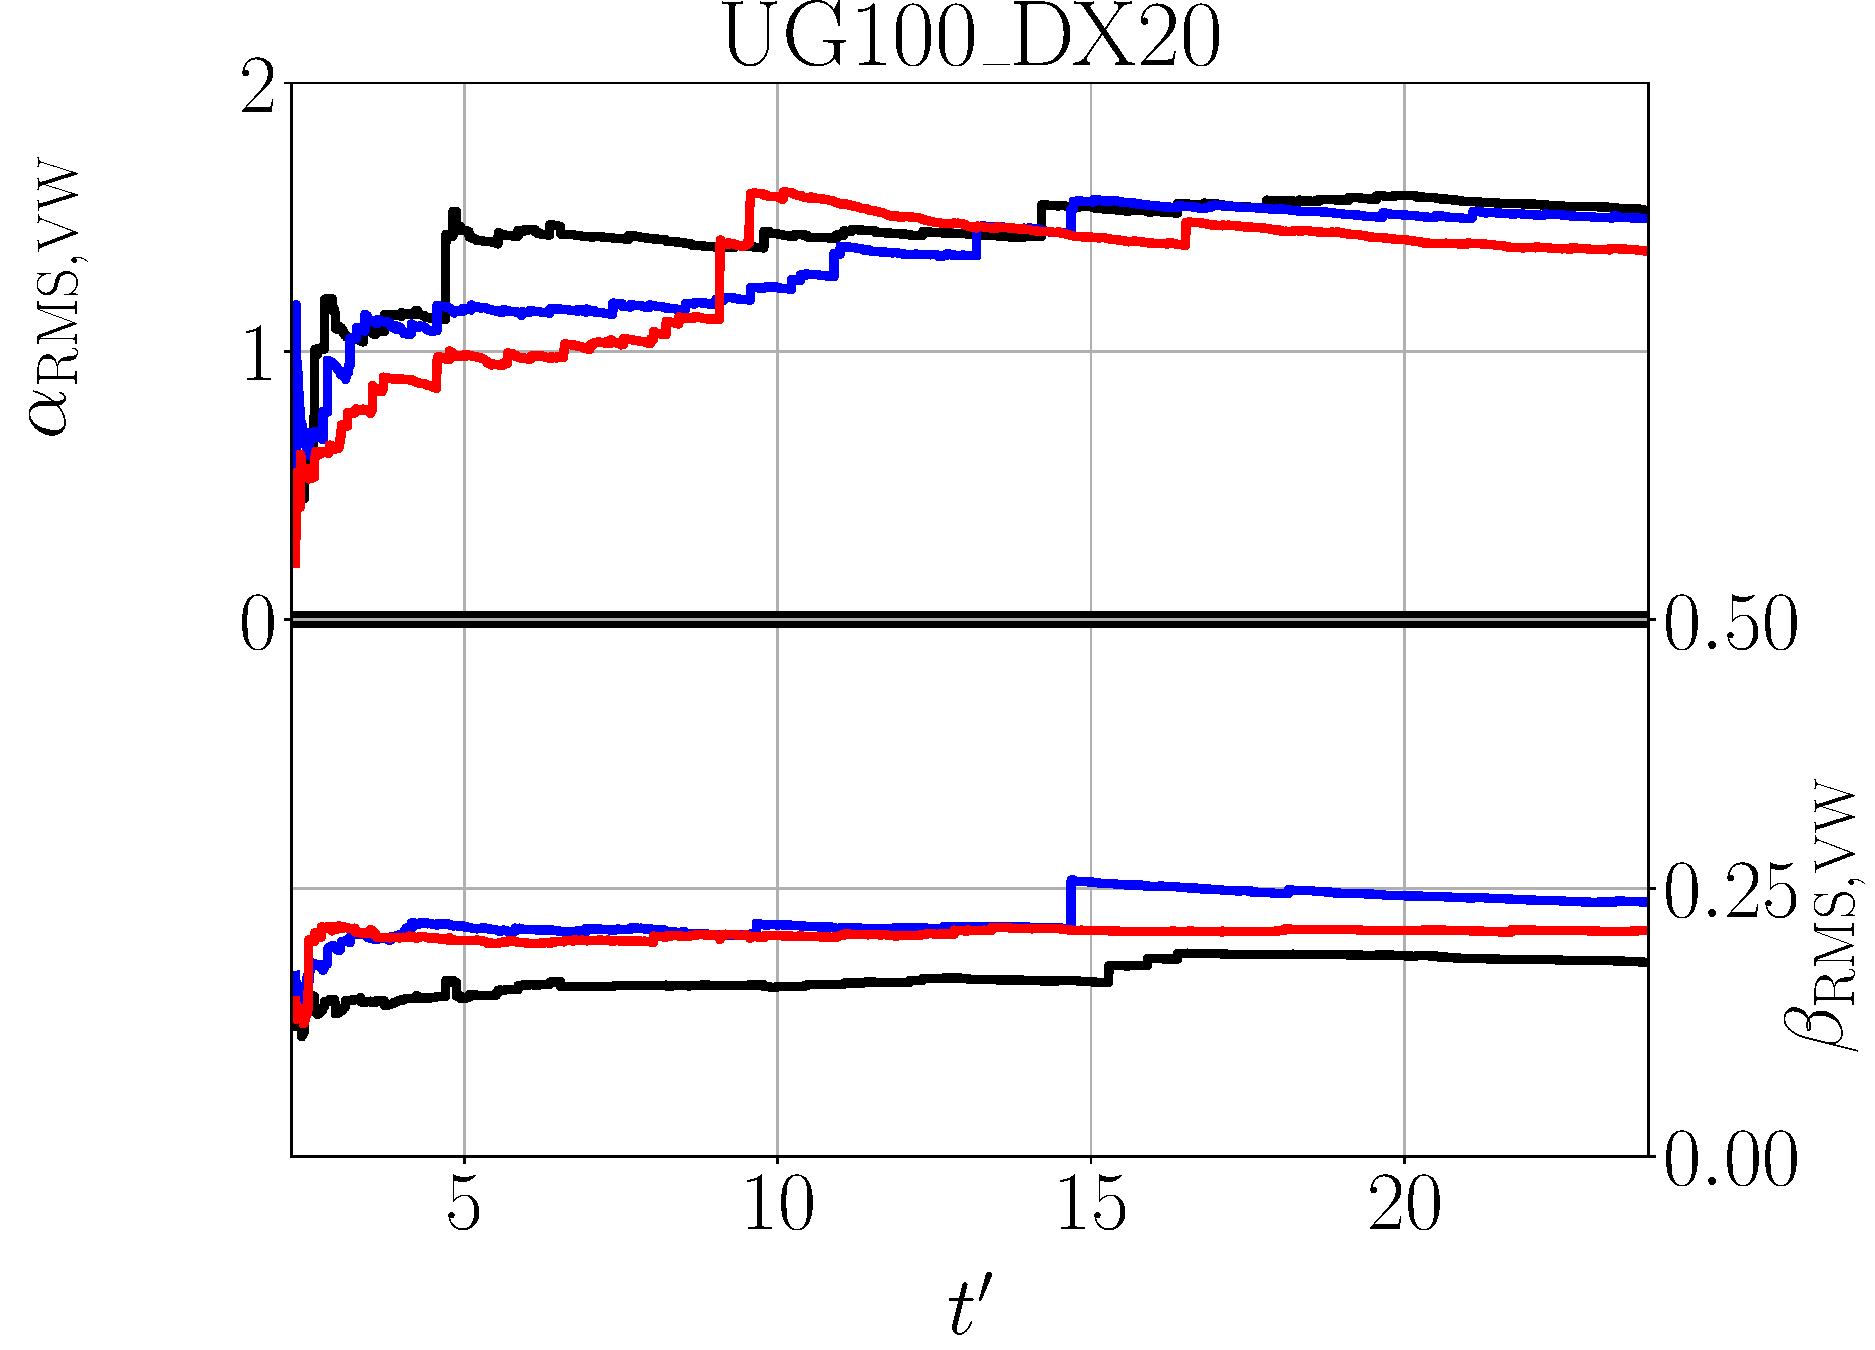
\includegraphics[width=0.3\textwidth]{./part2_developments/figures_ch5_resolved_JICF/SPRAY_characterization/deformation_establishment/establishment_UG100_DX20_rms}
   \hspace*{-0.1in}
   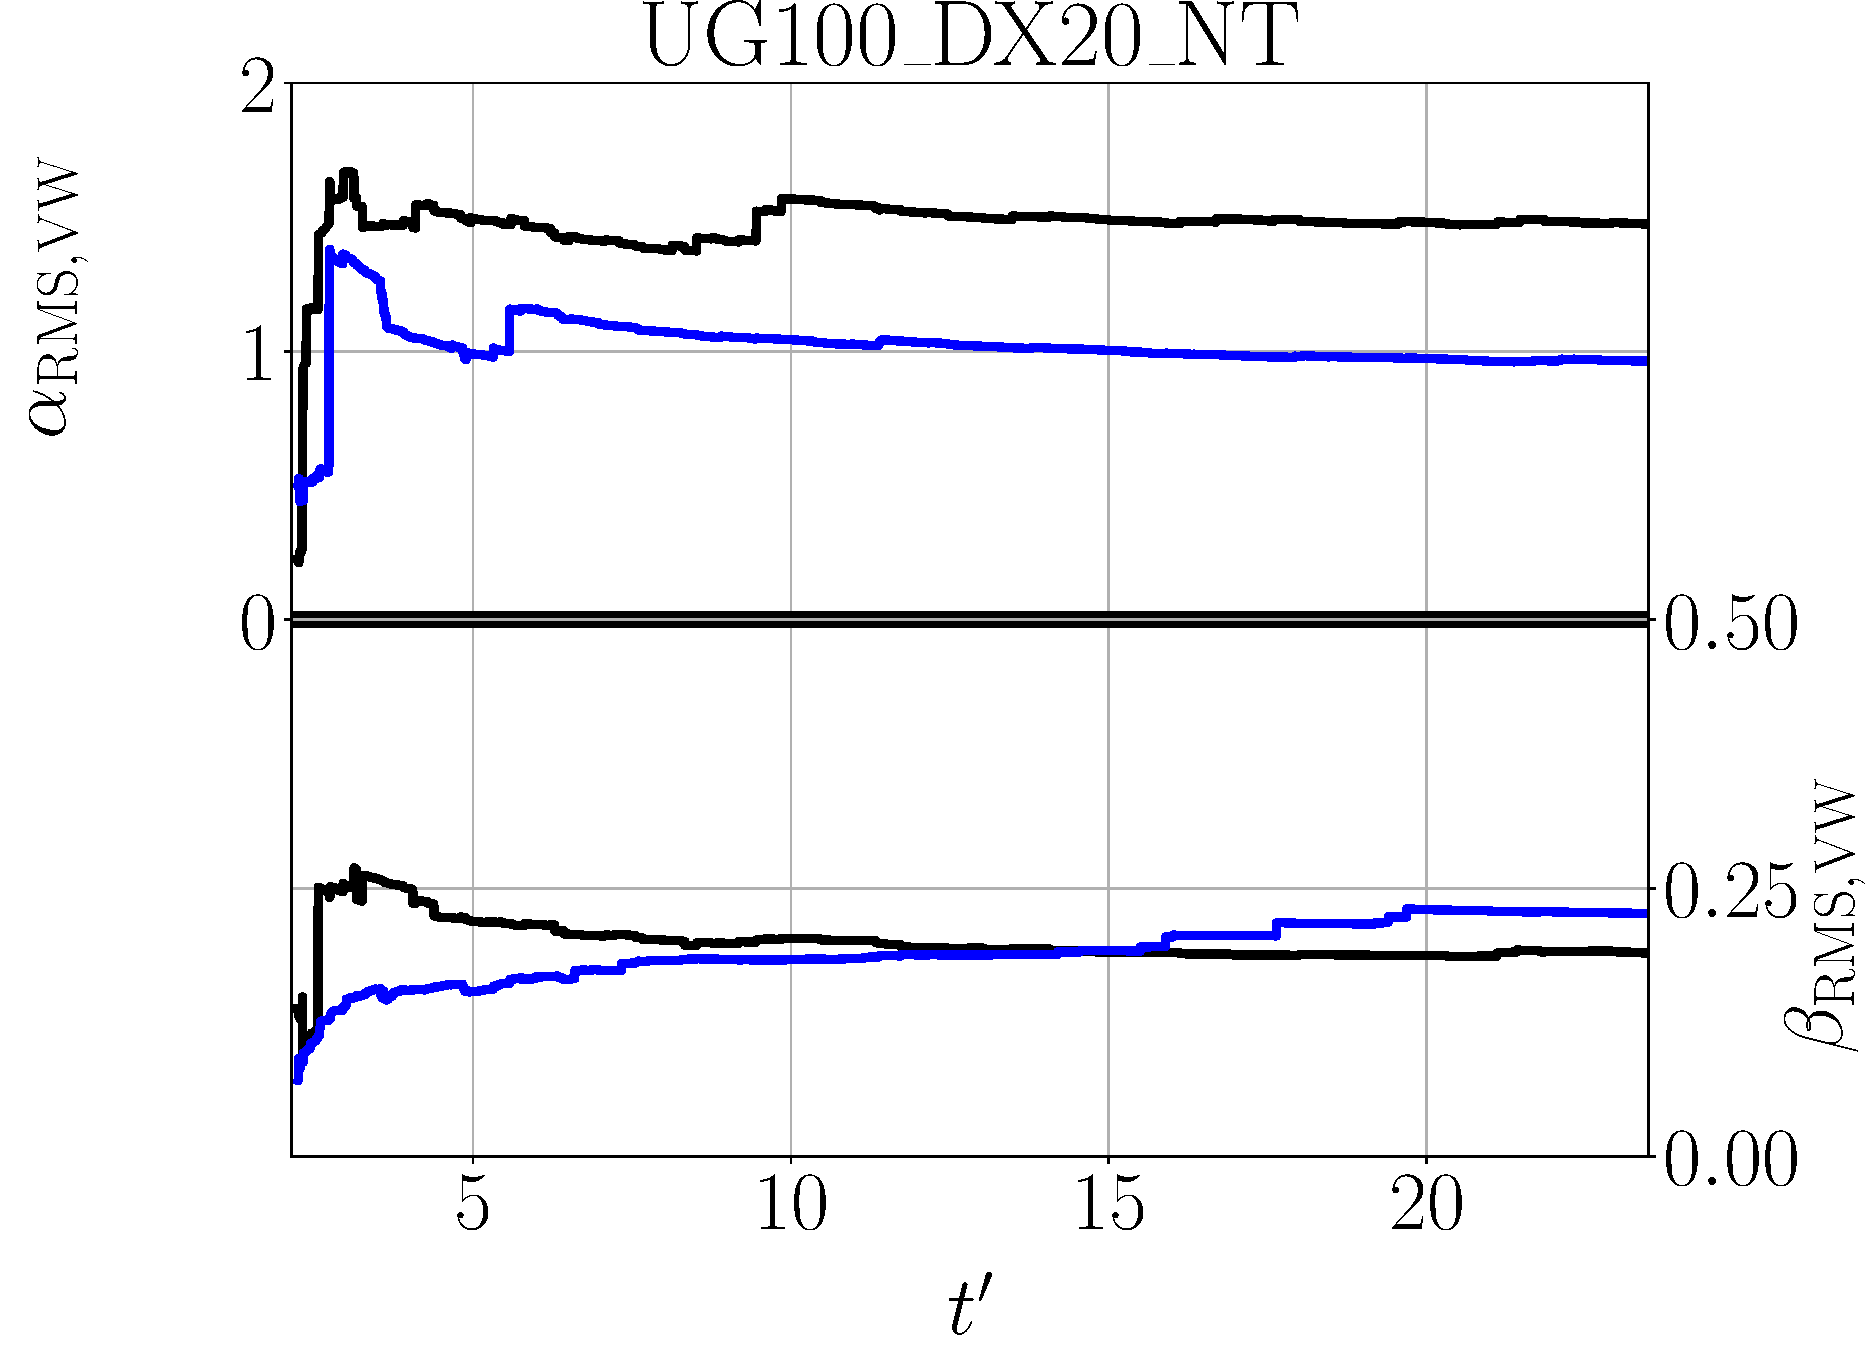
\includegraphics[width=0.3\textwidth]{./part2_developments/figures_ch5_resolved_JICF/SPRAY_characterization/deformation_establishment/establishment_UG100_DX20_NT_rms}
   \caption{Establishment of RMS deformation parameters for each case.}
\label{fig:app_spray_deformation_establishment_rms}
\end{figure}
